\documentclass[11pt,a4paper]{article}

\usepackage[utf8]{inputenc}
\usepackage[T1]{fontenc}
\usepackage[english]{babel}
\usepackage{geometry}
\geometry{a4paper, top=3cm, bottom=3cm, left=2.5cm, right=2.5cm}
\usepackage{graphicx}
\usepackage{hyperref}
\usepackage{listings}
\usepackage{xcolor}
\usepackage{booktabs}
\usepackage{float}

\lstset{
    language=Python,
    basicstyle=\ttfamily\footnotesize,
    keywordstyle=\color{blue},
    stringstyle=\color{red},
    commentstyle=\color{green!60!black},
    numbers=left,
    numberstyle=\tiny,
    stepnumber=1,
    numbersep=8pt,
    backgroundcolor=\color{gray!10},
    showstringspaces=false,
    frame=single,
    breaklines=true
}

\hypersetup{
    colorlinks=true,
    linkcolor=black,
    filecolor=magenta,      
    urlcolor=blue,
    pdftitle={Volvo IT Incident Management Report},
}

\begin{document}

% ---------------- FRONTESPIZIO ----------------
\begin{titlepage}
    \centering
    \vspace*{1cm}

    {\LARGE \scshape Università degli Studi di Milano \par}
    \vspace{2cm}

    
\includegraphics[width=8cm]{pictures/unimi.pdf}
    \vspace{2cm}

    % Titolo del progetto 
    {\Huge \bfseries Business Information Systems \\ exam call \par}
    \vspace{2cm}

    {\Large \bfseries Gianluca Pironato - 47257A \par}
    \vspace{1.5cm}

    {\large 29th of June 2026 \par}

    \vfill
\end{titlepage}

% ---------------- INDICE ----------------
\newpage
\tableofcontents
\newpage

% ---------------- CORPO DEL REPORT ----------------

\section{Introduction} 
The management of IT incidents is fundamental to minimize the periods of system inactivity and to guarantee the continuity of business operations. Volvo IT Belgium uses a system that generates a huge quantity of event data recorded within log archives. The main goal of process mining is to extract process models directly from these event logs, with the aim of optimizing the organizational procedures.

\section{Description of the case study}
Volvo IT Belgium provides IT infrastructure and assistance services to the Volvo Group. For the governance of technical problems and incidents, they use an IT service management system that registers every mutation of tickets' status and reassignment of an incident, from its origination to its definitive closure.

The incident management procedure relies on three support levels. In an ideal scenario, incidents obtain rapid resolution at the initial line of support but complications can bring to escalation towards more specialized teams. Although this practice represents a standard methodology, the empirical data are here used to investigate potential inefficiencies.

The main problematic aspects subjected to the present investigation incorporate possible delays due to escalation abuses and the presence of ping-pong behaviours, wherein tickets are iteratively transferred among specific support groups without advancing toward a definitive resolution. These redundant transmissions are prone to generating inflated waiting durations and failures, potentially deviating the organization from its objectives of efficiency and performance. Furthermore, the present case study evaluates the process execution consistency across various departments, in order to comprehend whether they operate in conformity with the normative incident lifecycle or if specific groups introduce procedural deviations.

\subsection{Dataset overview}

The event log is provided in the XES format and it is structured to capture the complete lifecycle of VINST IT incidents:
\begin{itemize}
    \item the entire \textbf{Log} represents the collection of IT incidents/traces handled by Volvo IT Belgium. Within the log;
    \item each \textbf{Trace} corresponds to a single IT incident, uniquely identified by its \texttt{concept:name} attribute (e.g., \texttt{1-718915746}), and contains the chronologically ordered sequence of the activities/events performed leading to its resolution; \item finally, each \textbf{Event} represents a single activity or status change within that specific incident. 
\end{itemize}
Each activity/event has several key attributes:
\begin{itemize}
    \item \textbf{Activity \& status}: \texttt{concept:name} defines the main status (e.g., \texttt{Accepted}, \texttt{Queued}), while \texttt{lifecycle:transition} indicates the sub-status (e.g., \texttt{In Progress});
    \item \textbf{Temporal data}: \texttt{time:timestamp} records the exact execution time, which can be used for calculating durations and waiting times, even though a complete dataset would provide also \texttt{start-timestamp} and \texttt{completion-timestamp} for each event;
    \item \textbf{Organisational context}: \texttt{org:group} explicitly identifies the assigned support team and its hierarchical tier (e.g., 1st line, or 2nd line indicated by suffixes like \texttt{2nd});
    \item \textbf{Metadata}: details such as incident \texttt{impact}, the affected \texttt{product}, and geographical locations (\texttt{resource/organization country}).
\end{itemize}

\section{Organisational goals}
To effectively analyse and improve incident management at Volvo IT Belgium, it is necessary to align the process mining findings with the company's objectives. These can be categorized into strategic, operational, and tactical levels, representing the high-level business aims, the functional processes required to achieve them and the specific daily tasks that compose those processes, respectively.

\subsection{Strategic goals}
At the strategic level, the primary objective of Volvo IT is to guarantee the high availability and reliability of IT services to support the core business operations of the Volvo Group. This means minimizing system downtime and ensuring business continuity and maximizing end-user productivity and satisfaction by providing a seamless and responsive IT support experience.

\subsection{Operational goals}
To pursue the strategic aims, the IT support functions must operate efficiently. The operational goals focus on streamlining the incident management lifecycle across all support tiers. Key objectives include maximizing the first-line resolution rate, minimizing unnecessary escalations to specialized second and third-line teams, and eliminating redundant handovers (ping-pong behaviours) that might cause bottlenecks and inflate overall resolution times.

\subsection{Tactical goals}
At the tactical level, the focus shifts to the specific activities and tasks performed by human operators within the VINST system. Tactical goals include establishing strict assignment criterias to prevent bouncing tickets between groups and standardizing status updates to ensure that all departments conform to the defined procedural lifecycle without unauthorized deviations or cyclic loops.

\newpage

\section{Project development}

\subsection{The knowledge uplift trail - KUT}
The analysis follows a structured knowledge uplift trail to extract actionable insights from the raw event log. This process is designed to filter traces considered noise or useless data, to identify potential bottlenecks along with their related causes and to look for procedural deviations.

The methodology consists of four main phases: first, data preparation and log segmentation isolate interesting incidents and group traces by their maximum level of escalation; second, an algorithm detects and quantifies ping-pong handover behaviours across different support groups; third, a conformance analysis is conducted using the Heuristics Miner to generate an ideal reference model and, finally, these findings are synthesized to propose concrete improvement opportunities.


\begin{table}[H]
    \centering
    \renewcommand{\arraystretch}{1.3} % Aumenta leggermente lo spazio verticale
    \small % Rimpicciolisce il testo per far stare tutto nella pagina
    \begin{tabular}{|p{0.7cm}|p{2.5cm}|p{2.8cm}|p{3.5cm}|p{2cm}|p{1.8cm}|}
        \hline
        \textbf{Step} & \textbf{Input} & \textbf{Analytics} & \textbf{Acquired knowledge} & \textbf{Type of knowledge} & \textbf{Output} \\
        \hline
        1 & Raw event log & Data cleaning \& segmentation & Segmentation of incidents by escalation depth and removal of automated system noise. & Descriptive & 1st, 2nd and 3rd-level logs \\
        \hline
        2 & Cleaned segment logs & Pattern matching (A $\rightarrow$ B $\rightarrow$ A ) & Identification of worst initiator groups. & Diagnostic & Bottleneck metrics and initiator distributions \\
        \hline
        3 & Unified log (excluding ping-pongs) & Process discovery with Heuristics Miner & Extraction of an ideal incident management lifecycle. & Descriptive & Ideal Petri Net of the reference model \\
        \hline
        4 & Unified log (including ping-pongs) & Data filtering & Isolation of traces handled exclusively by specific critical groups vs baseline. & Descriptive & 3 variant sub-logs \\
        \hline
        5 & Variant sub-logs and reference model & Conformance checking with Token-Based replay & Distinction between organizational inefficiency and procedural non-conformance. & Diagnostic & Fitness scores and conformance insights \\
        \hline
        6 & Fitness scores and temporal data & Prescriptive analysis & Translation of algorithmic anomalies into concrete operational recommendations. & Prescriptive & Improvement opportunities \\
        \hline
    \end{tabular}
\end{table}

\subsection{Dataset segmentation}
The first requirement of the project is to investigate the frequency of incident escalations across the support levels. This metric is a result easily obtained as a direct product of the log segmentation. Therefore, the first step is to partition the dataset into mutually exclusive subsets based on the highest level reached by each IT incident. Based on the \texttt{org:group} attribute, the traces are classified into three independent event logs:
\begin{enumerate}
    \item \textbf{First-level support log}: traces containing events handled exclusively by first-line operators (no occurrence of \texttt{"2nd"} or \texttt{"3rd"} in any event's \texttt{org:group}).
    \item \textbf{Second-level escalation log}: traces that required an escalation to the second line, but were resolved without reaching the third line (at least one occurrence of \texttt{"2nd"}, but zero occurrences of \texttt{"3rd"}).
    \item \textbf{Third-level escalation log}: traces that reached the highest level of complexity, requiring intervention from third-line specialists (at least one occurrence of \texttt{"3rd"}).
\end{enumerate}

The code in \texttt{segmentation\_and\_escalation\_stats.py} demonstrates the implementation of this classification logic, ensuring that metadata and extensions from the original XES file were properly preserved in the output segments using PM4PY.

The execution of the script over the initial dataset resulted in the following distribution:

\begin{itemize}
    \item \textbf{Total traces}: 7554
    \item \textbf{First-level support log}: 4546
    \item \textbf{Second-level escalation log}: 2464
    \item \textbf{Third-level escalation log}: 544
\end{itemize}

\subsection{Escalation frequency of IT incidents and data filtering}

To answer the request on escalation frequency, the above trace counts were converted into frequencies over the full population of 7554 incidents:

\begin{itemize}
    \item \textbf{First-line resolution frequency} (no escalation): $\frac{4546}{7554}=60.18\%$
    \item \textbf{Escalation frequency to specialised teams} (2nd and/or 3rd): $\frac{2464+544}{7554}=39.82\%$
    \item \textbf{Second-line-only escalation frequency}: $\frac{2464}{7554}=32.62\%$
    \item \textbf{Third-line escalation frequency}: $\frac{544}{7554}=7.20\%$
\end{itemize}


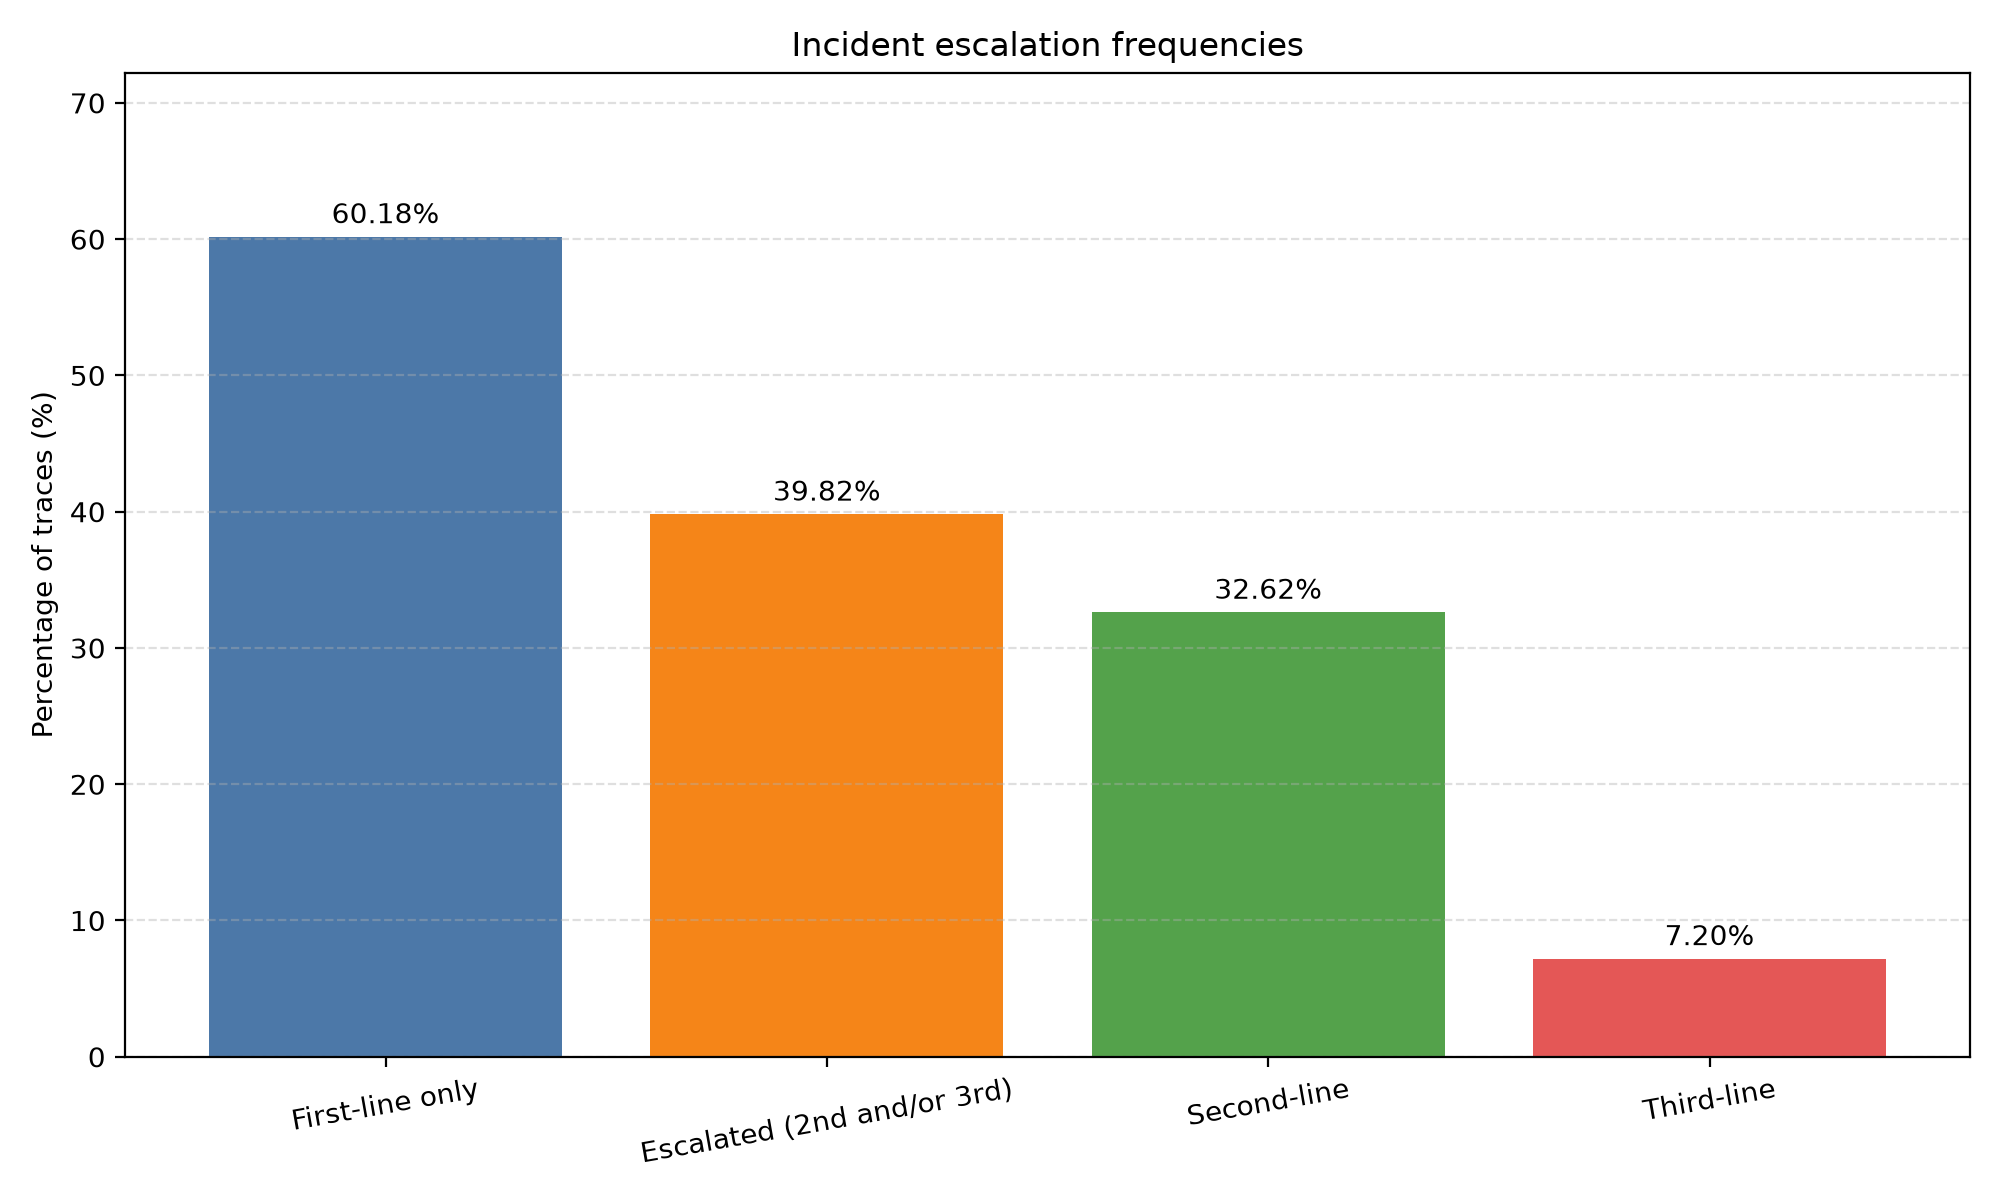
\includegraphics[width=0.9\textwidth]{pictures/escalation_frequency.png}

At this point we can state that while the majority of the incidents are successfully resolved by first-level technicians, a significant portion requires further escalation. 

To understand the impact of the operational differences between the support tiers, an analysis of the incident lead times (total duration from the first to the last timestamp of each trace) was conducted on the initial segments. The results are shown below.


    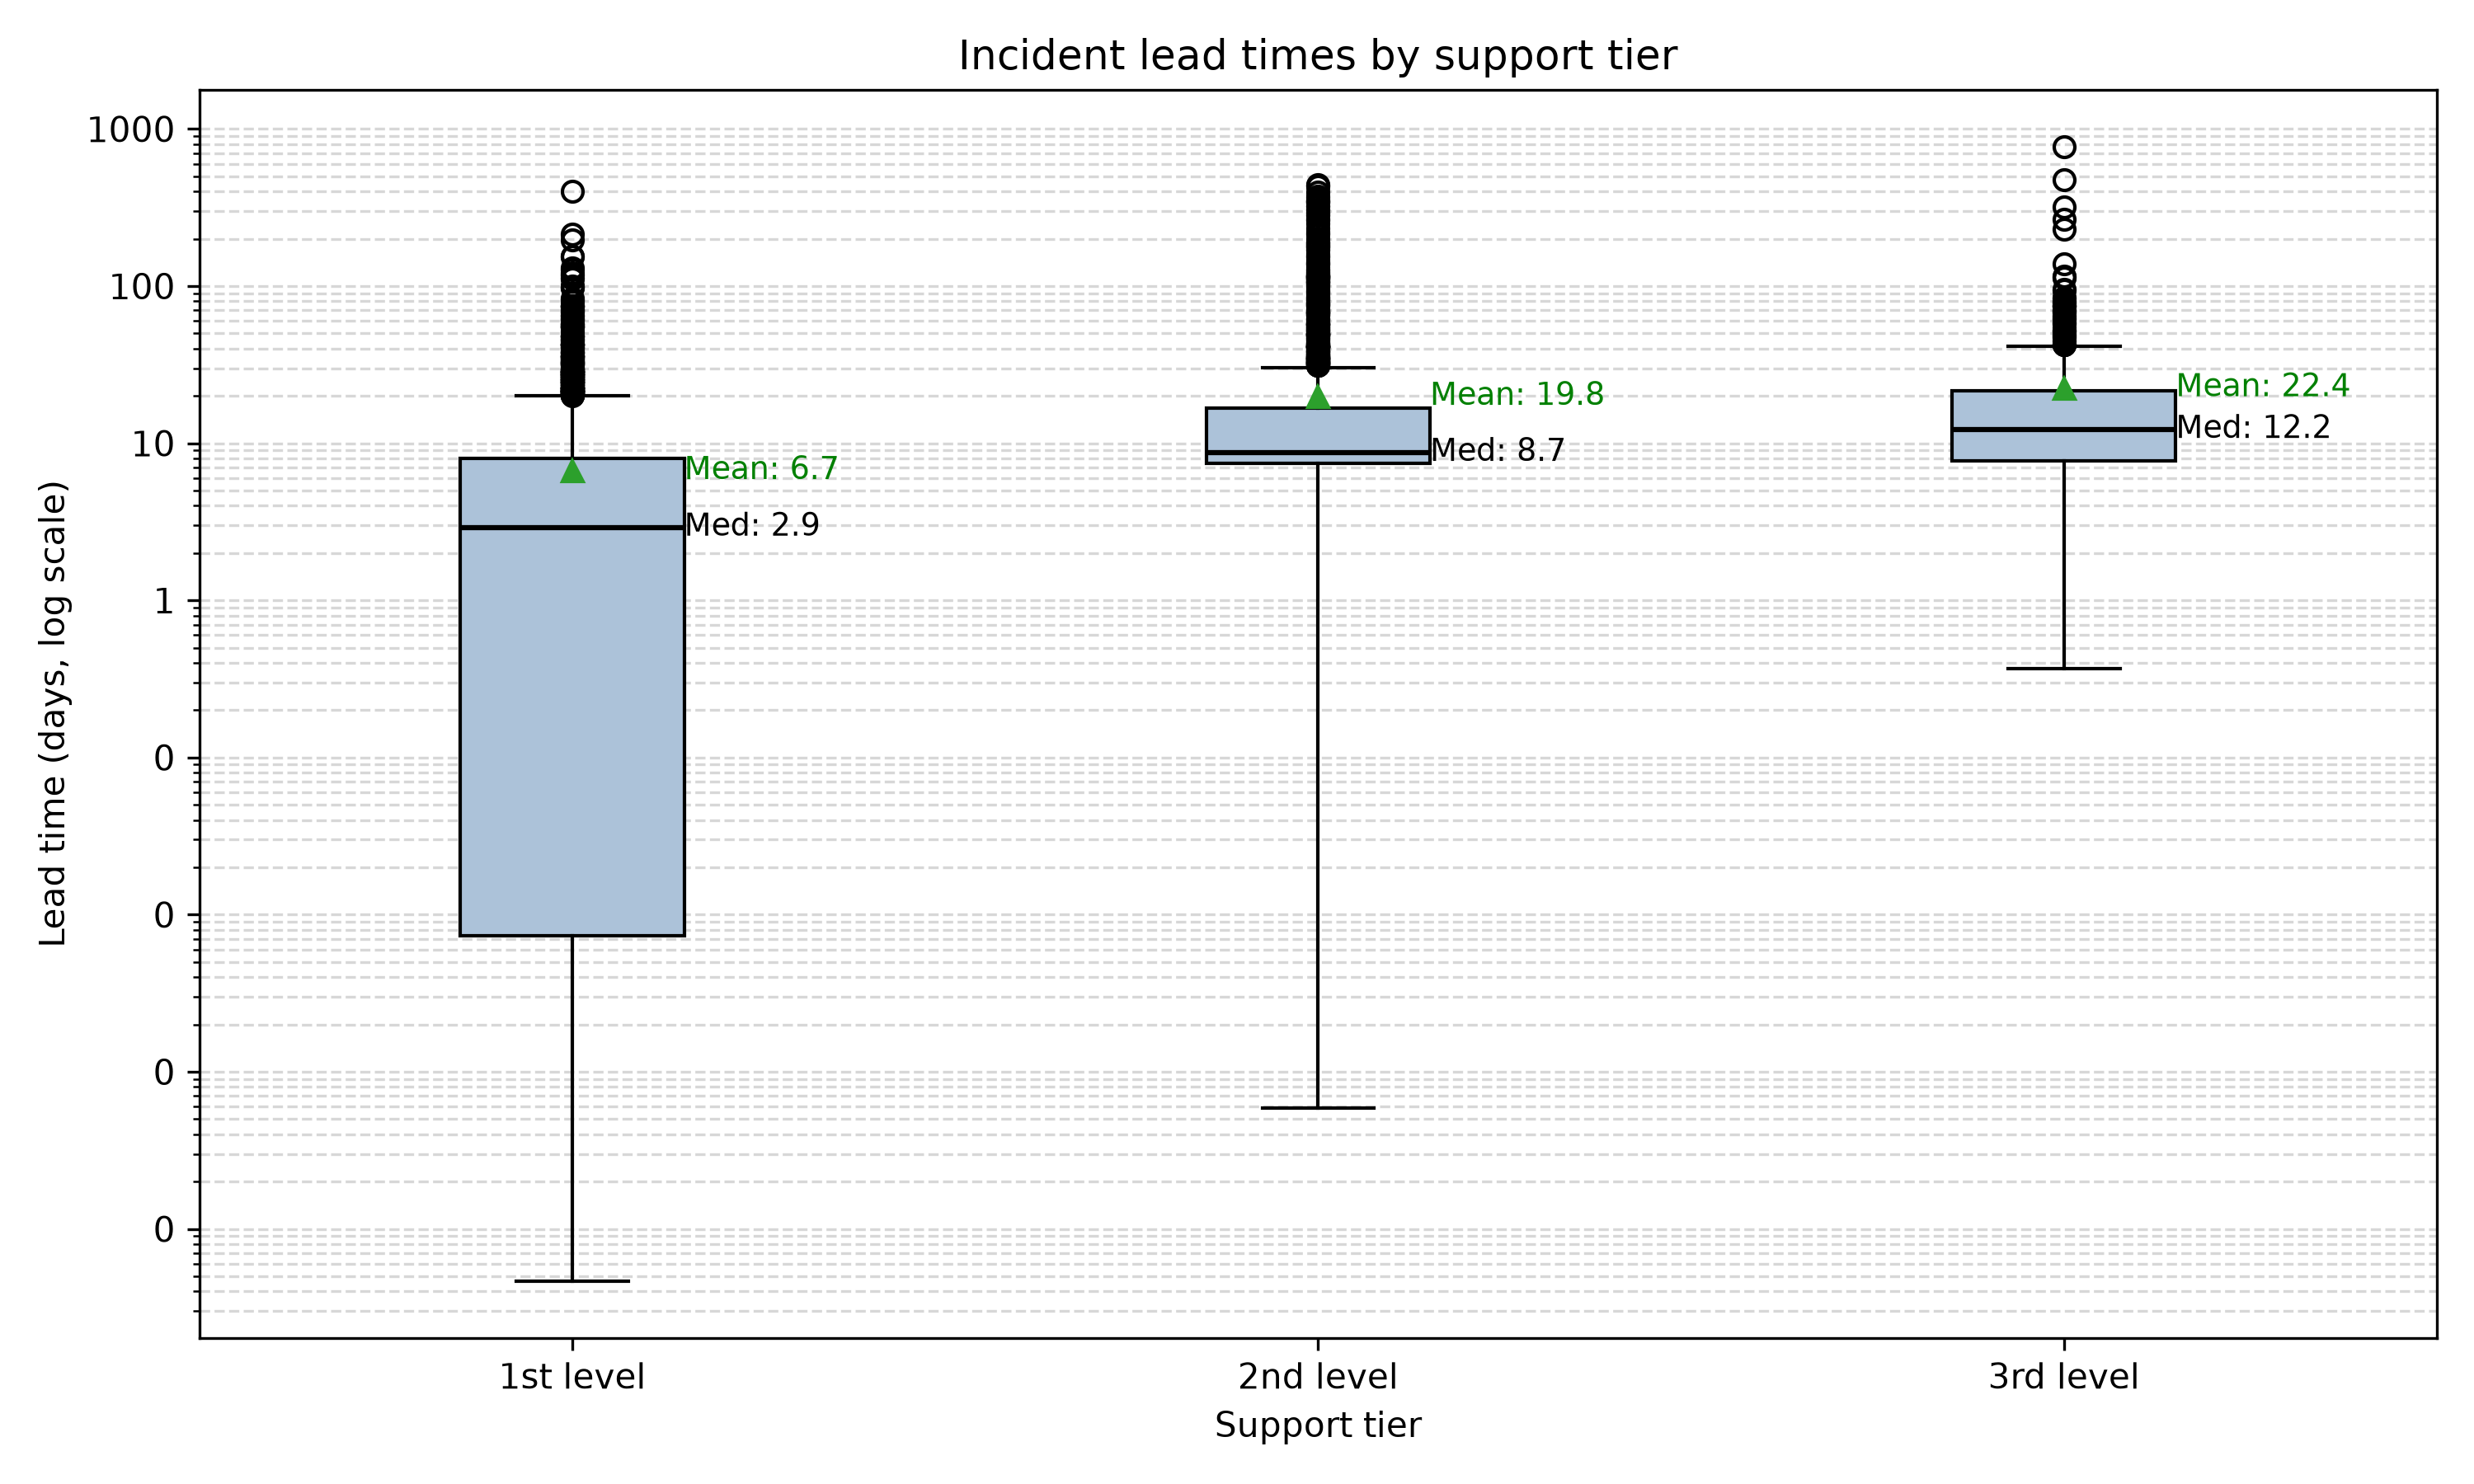
\includegraphics[width=0.9\textwidth]{pictures/lead_time_distribution_uncleaned.png}
    

The boxplot distribution reveals a logical progression in incident complexity across the escalation tiers. The median lead time increases consistently from 2.9 days in the first level to 8.7 days in the second, peaking at 12.2 days in the third level. However, a possible anomaly emerges within the first-level support data: while its mean is 6.7 days, the lower quartile stretches drastically toward the absolute minimum threshold; this massive concentration of extremely quick resolutions could be the result of systemic artifacts rather than standard human operations, giving a clear suggestion for data filtering.

The detailed distribution of traces per lead times is shown in the histogram below and it is characterized by a median of 2.91 days and an absolute mode of the distribution heavily concentrated in the very first bin, near zero.


    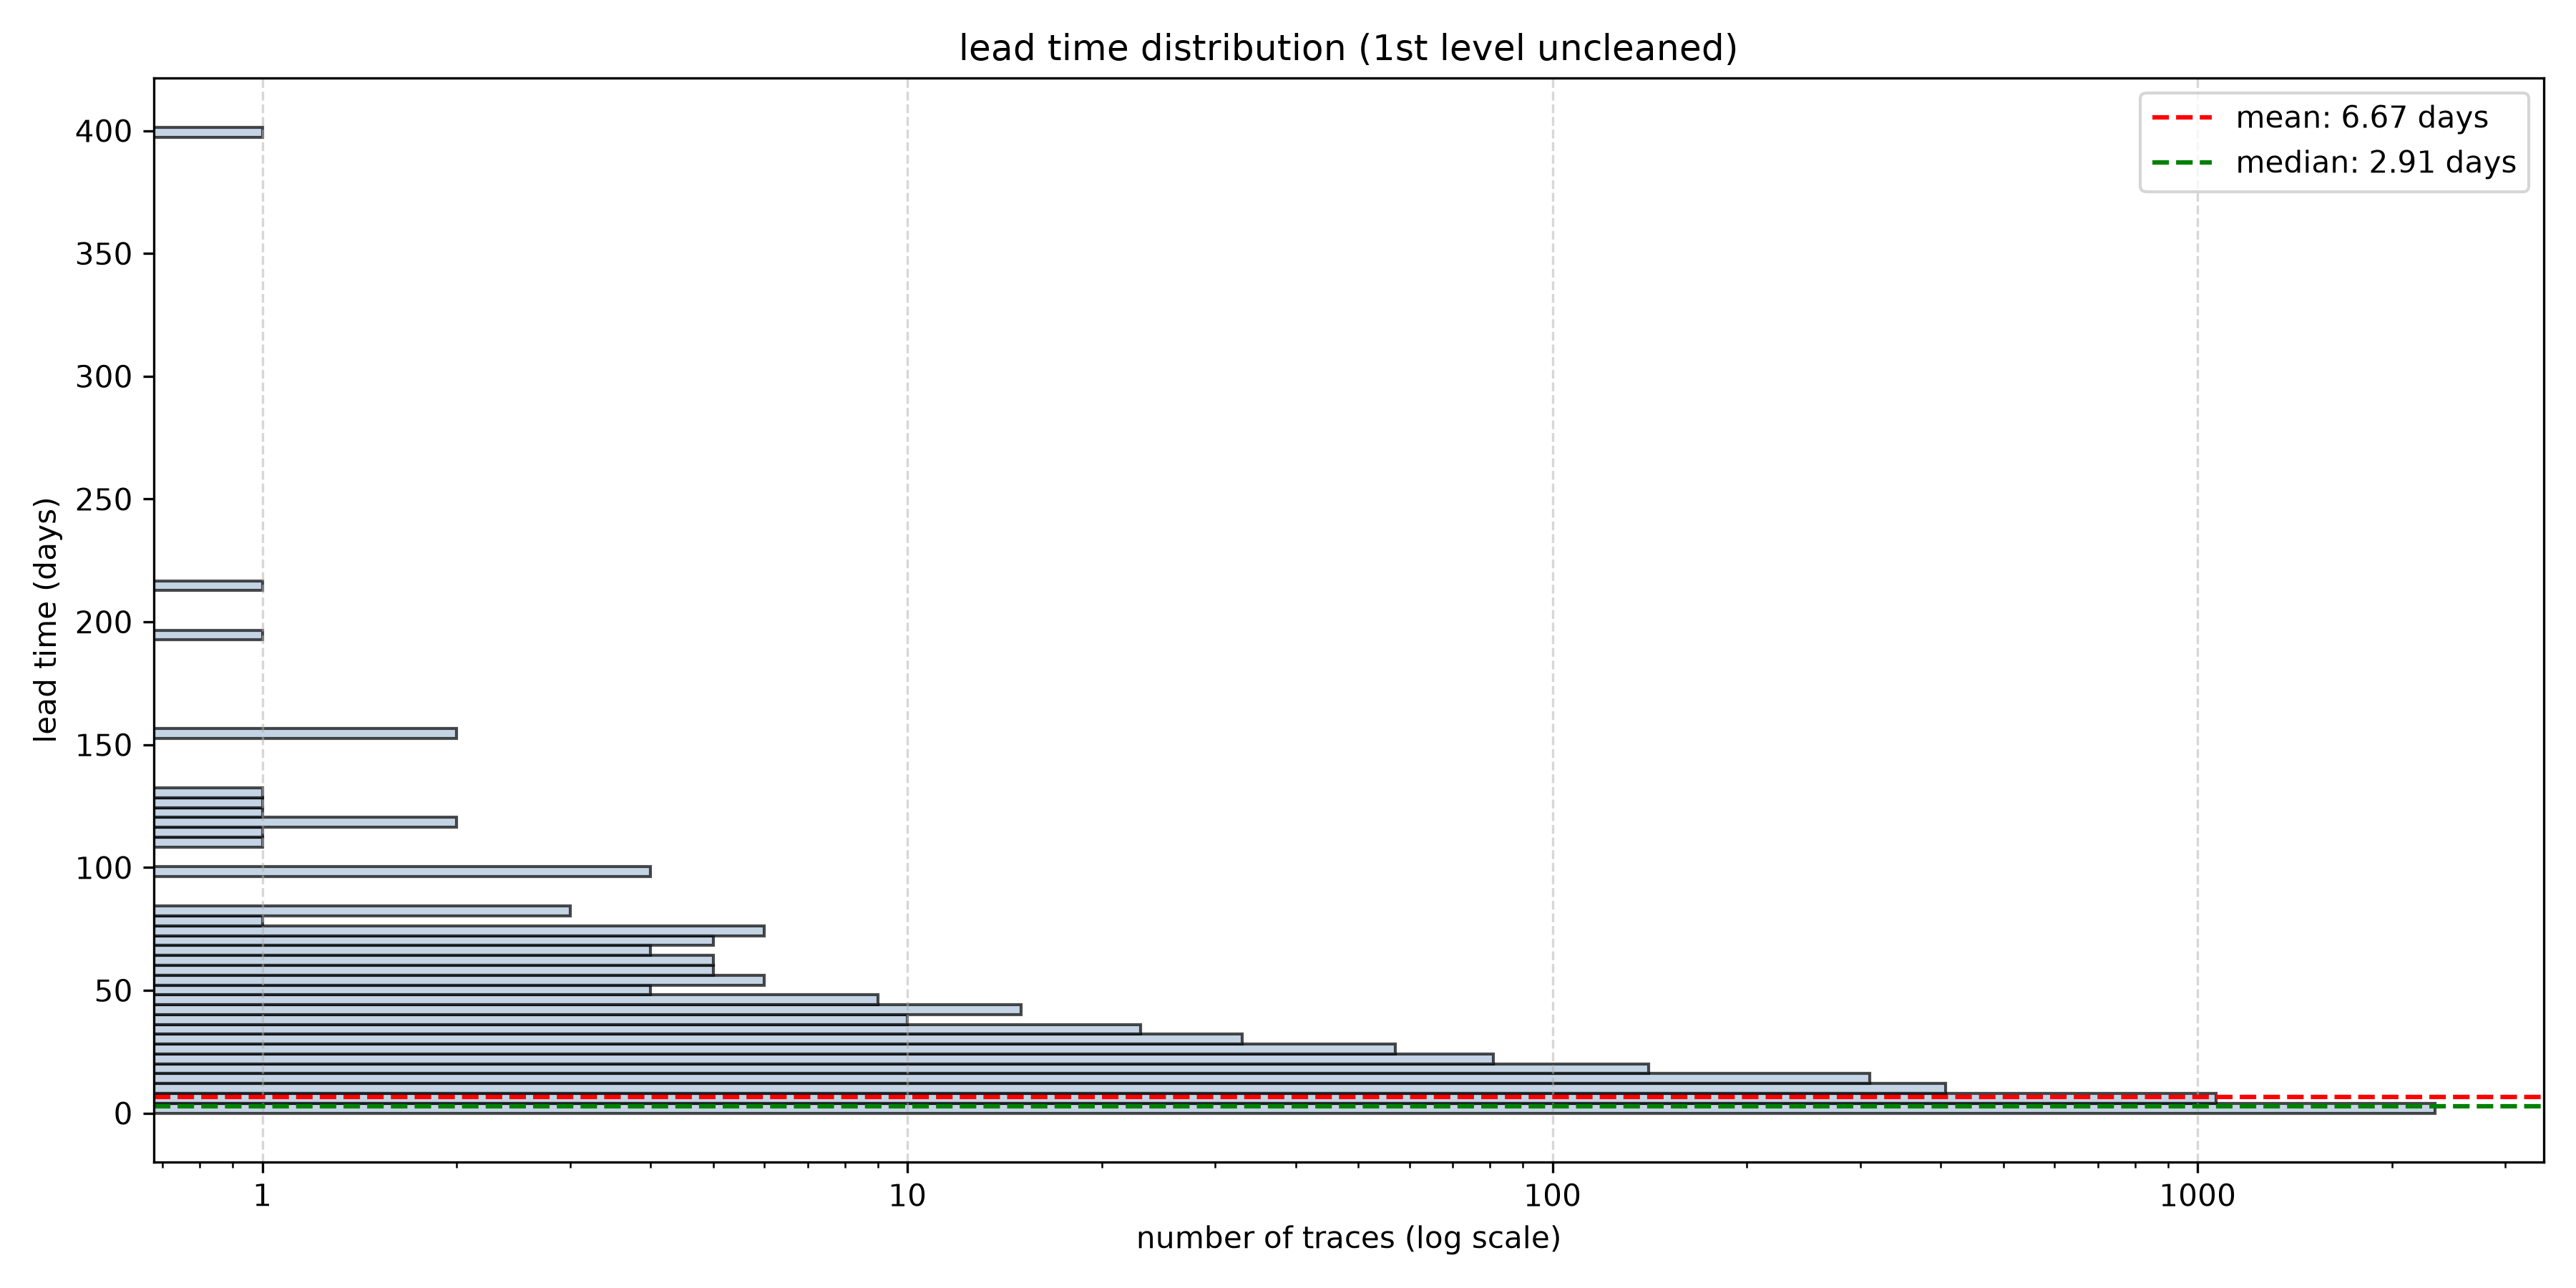
\includegraphics[width=0.9\textwidth]{pictures/distribution_1st_level_uncleaned.png}

This extreme concentration of quick resolutions has moved the focus of the exploratory analysis from the temporal dimension (lead time) to the structural dimension (the discrete number of events per trace), in order to investigate the nature of these incidents. The distribution by length ($n \le 10$) is the following:

\begin{table}[H]
    \centering
    \begin{tabular}{@{}cccc@{}}
        \toprule
        \textbf{Events (n)} & \textbf{1st level} & \textbf{2nd level} & \textbf{3rd level} \\ \midrule
        1 & 1 & 0 & 0 \\
        2 & 5 & 4 & 1 \\
        3 & 1722 & 36 & 3 \\
        4 & 569 & 259 & 46 \\
        5 & 322 & 90 & 12 \\
        6 & 407 & 291 & 41 \\
        7 & 292 & 209 & 69 \\
        8 & 259 & 269 & 45 \\
        9 & 192 & 152 & 47 \\
        10 & 131 & 142 & 41 \\ \bottomrule
    \end{tabular}
\end{table}

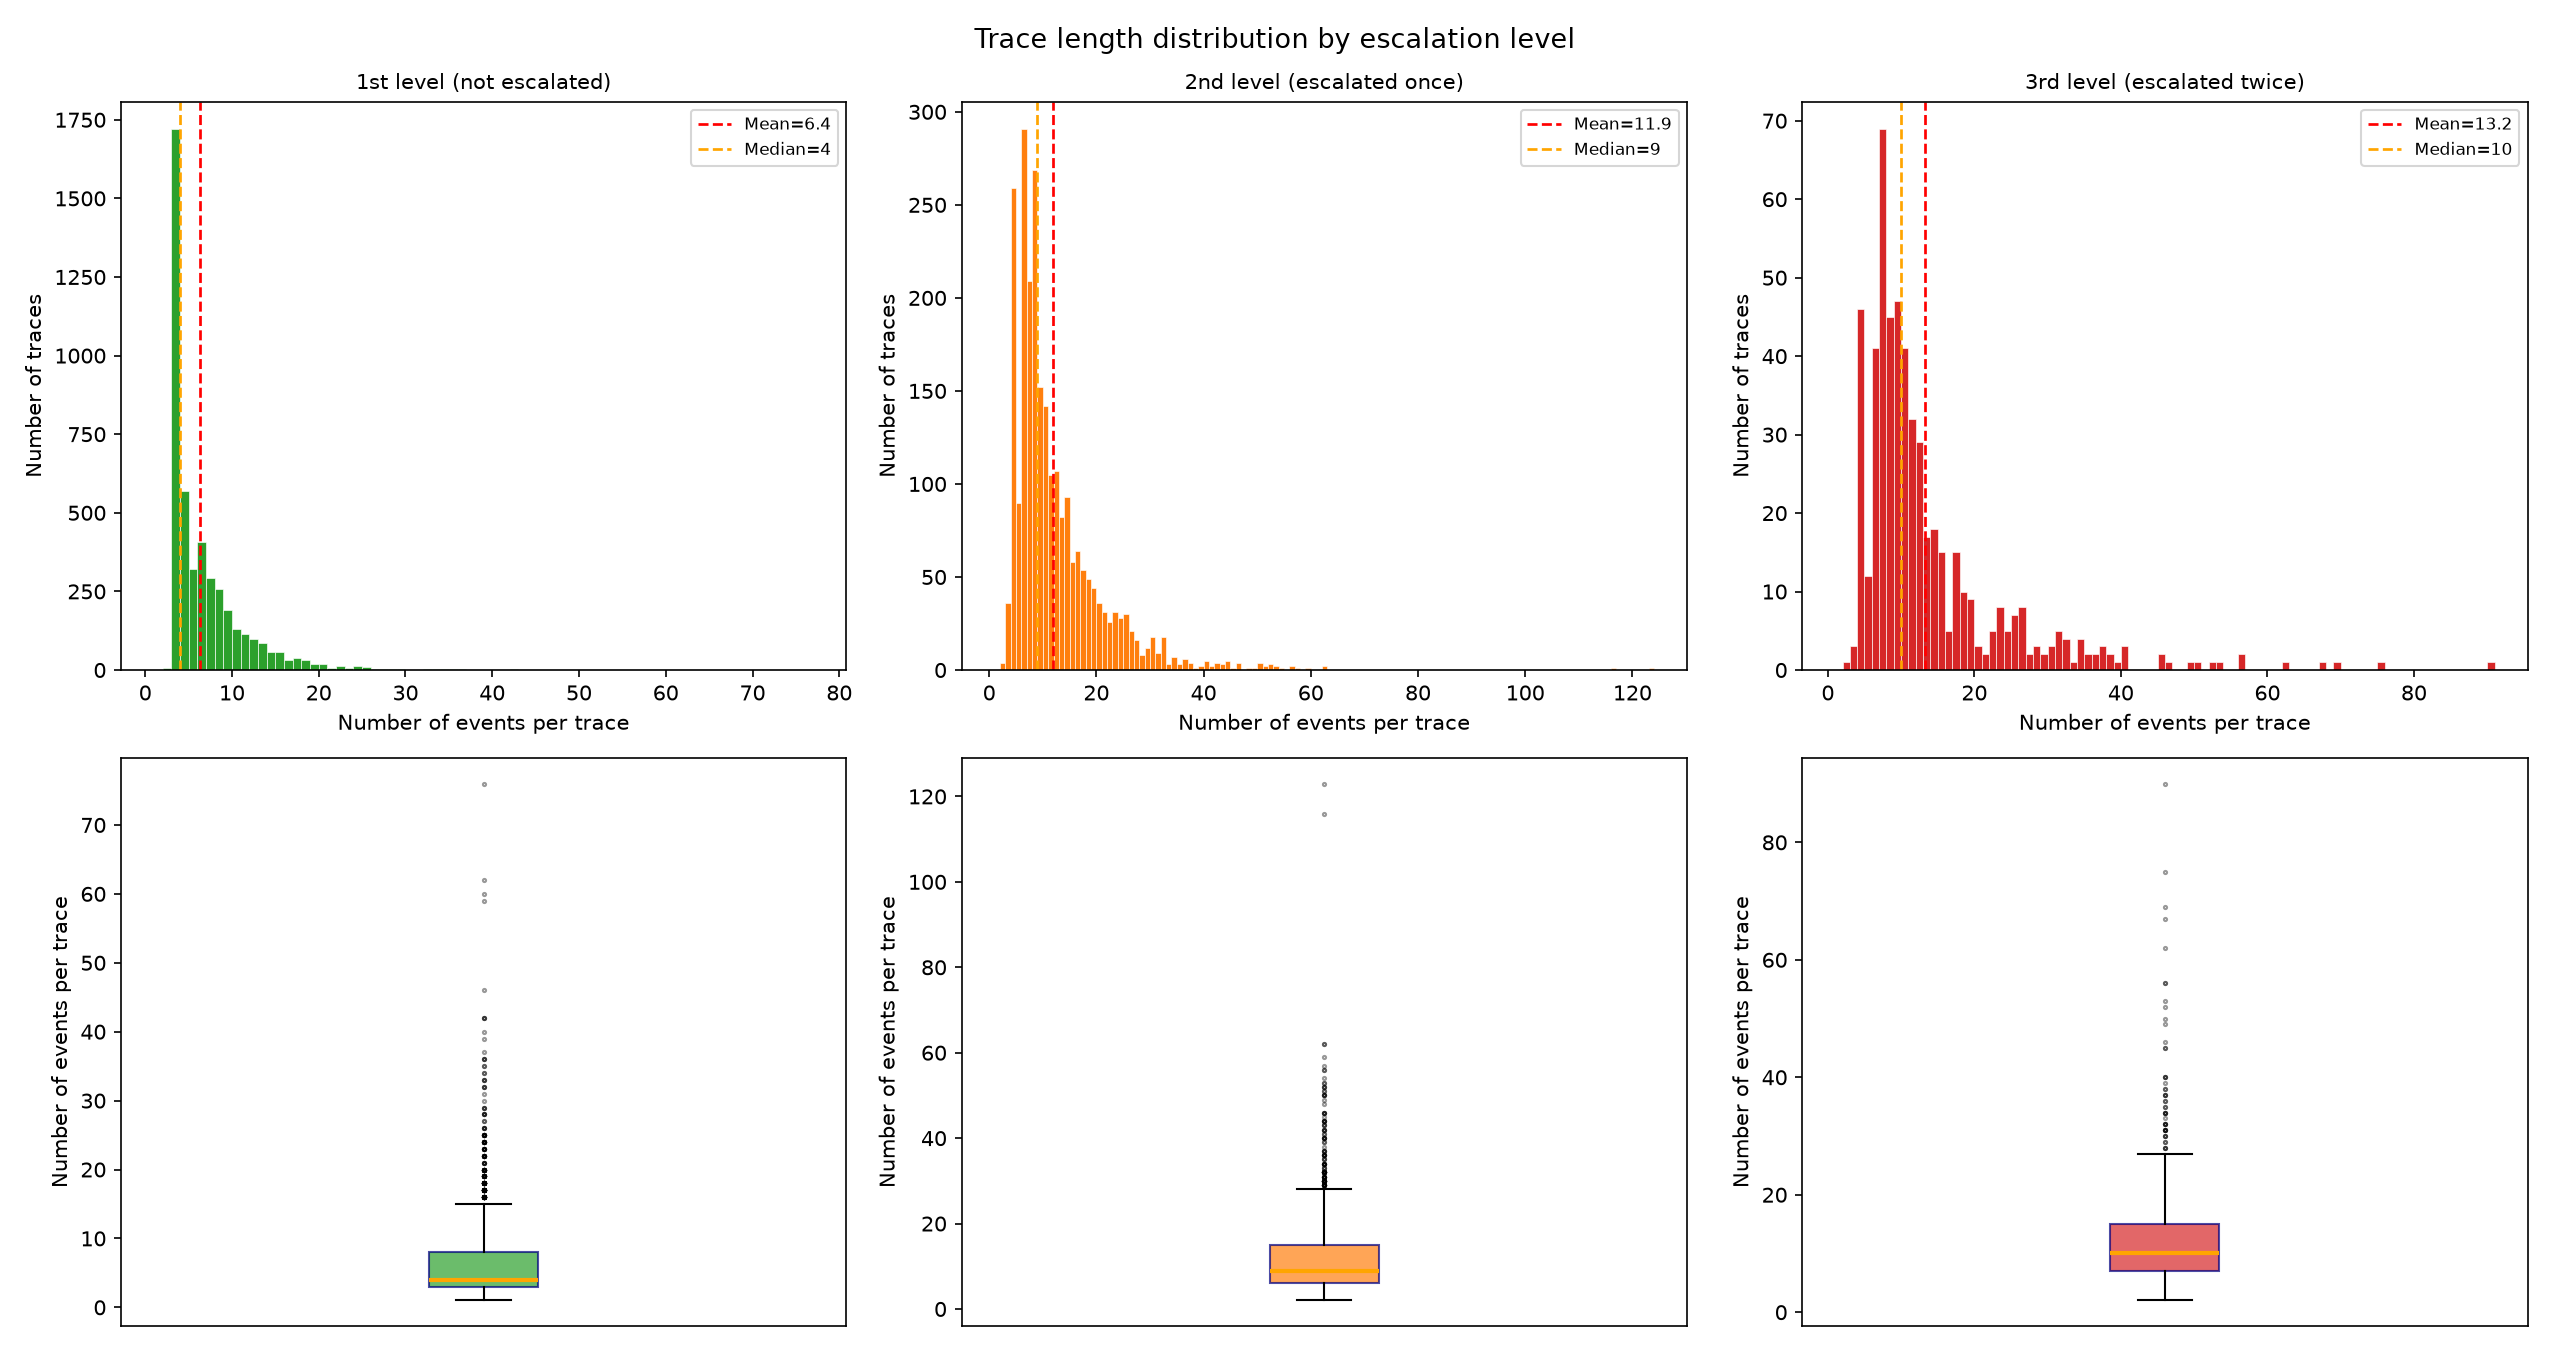
\includegraphics[width=0.9\textwidth]{pictures/dist_segments.png}

The data in the table reveal an exceptional amount of short traces which have the same exact number of events (3). These 1722 traces could be the ones also responsible for the very skewed distribution in terms of time duration. To formally validate the anomalous nature of this frequency, a Chi-square test was performed against a theoretical uniform distribution. The resulting p-value ($p < 0.001$) confirms that the frequency of 3-event traces is a statistical outlier, providing a mathematical foundation for their exclusion. Because of their shortness, such sequences hardly represent a human workflow involving diagnosis and resolution, and could be considered as noise (like automatic erroneous opened and almost instantly closed tickets).


    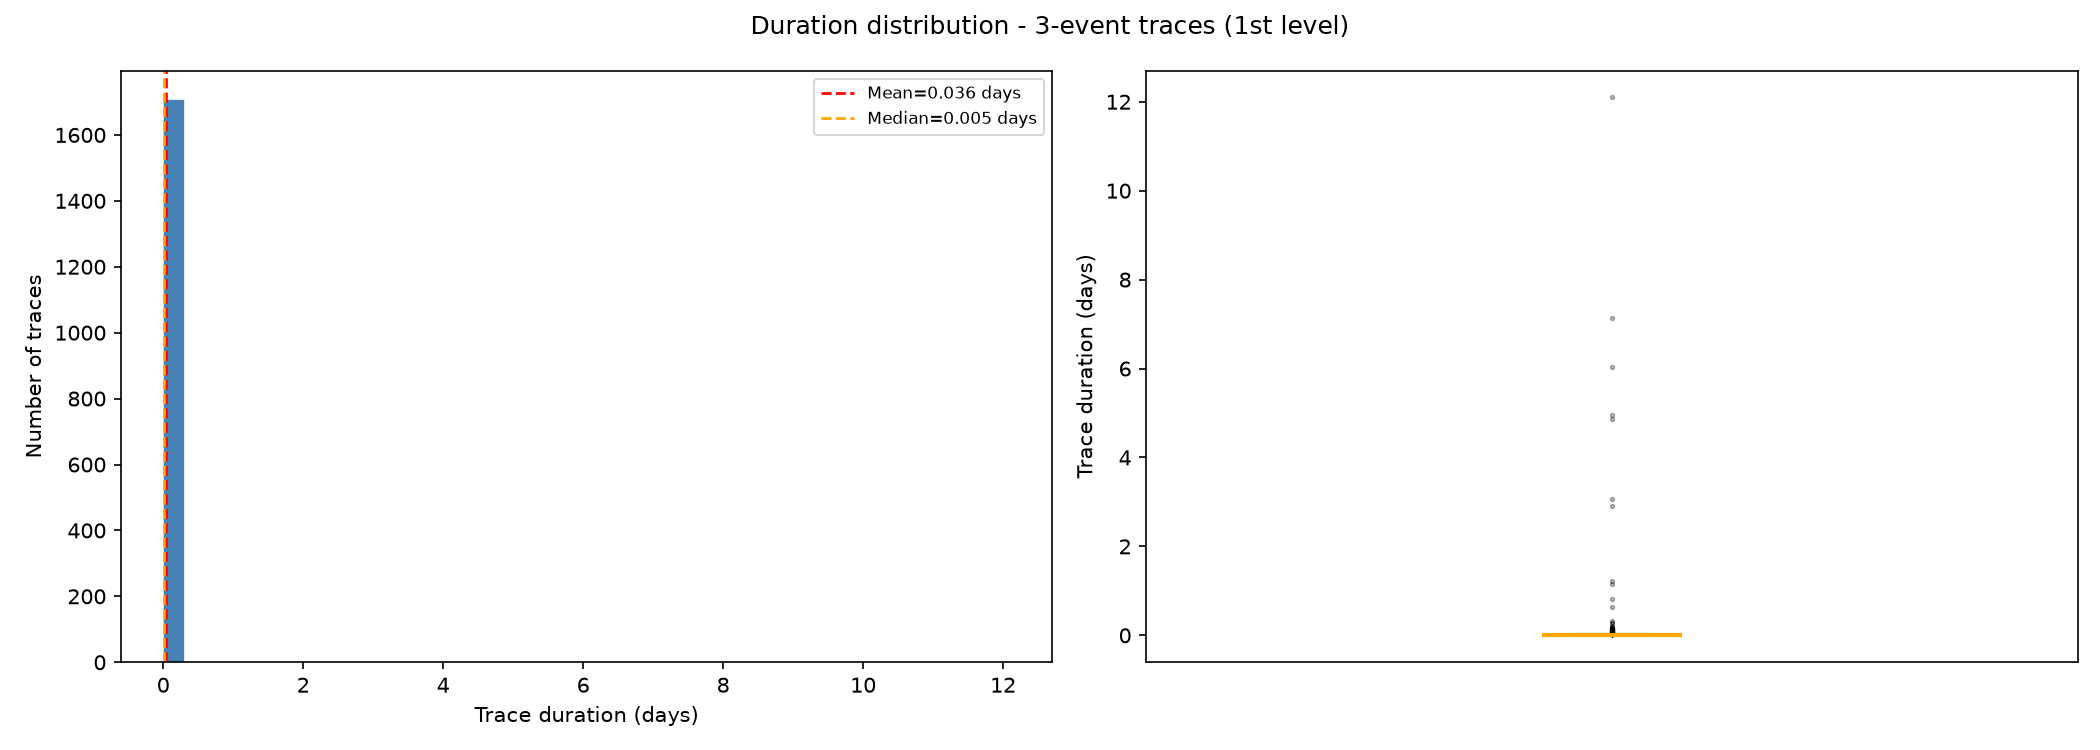
\includegraphics[width=0.9\textwidth]{pictures/dist_time_3event.png}

The results of the double check (\texttt{extract\_3event\_traces\_from\_1st\_level.py}) demonstrated a stark correlation: the vast majority of these 3-event traces have a very short resolution time, with a median of just 0.005 days (approximately 7 minutes). In the context of IT incidents management, a ticket resolved in such a time with only 3 status transitions can not reflect a human operational workflow involving diagnosis, assignment, and resolution.

Therefore, a filtering condition was established to remove all traces containing $\le 3$ events strictly from the first-level support log.

The execution of this targeted filtering strategy yielded the following final dataset dimensions:
\begin{itemize}
    \item \textbf{Input traces}: 4546
    \item \textbf{Removed traces}: 1728
    \item \textbf{Output traces}: 2818
\end{itemize}

Consequently, the cleaned first-level log provides a highly relevant baseline of 2818 traces, completely free from automated systemic noise. By eliminating these 1728 instances, the overall volume of the original dataset (7,554 traces) was lightened by approximately 22.88\%. After the phase of data filtering, the escalation frequencies of IT incidents have been recalculated.

The updated frequencies are the following ones:
\begin{itemize}
    \item \textbf{First-line resolution frequency} (no escalation): $\frac{2818}{5826} = 48.37\%$
    \item \textbf{Escalation frequency to specialized teams} (2nd and/or 3rd): $\frac{2464+544}{5826} = 51.63\%$
    \item \textbf{Second-line-only escalation frequency}: $\frac{2464}{5826} = 42.29\%$
    \item \textbf{Third-line escalation frequency}: $\frac{544}{5826} = 9.34\%$
\end{itemize}

    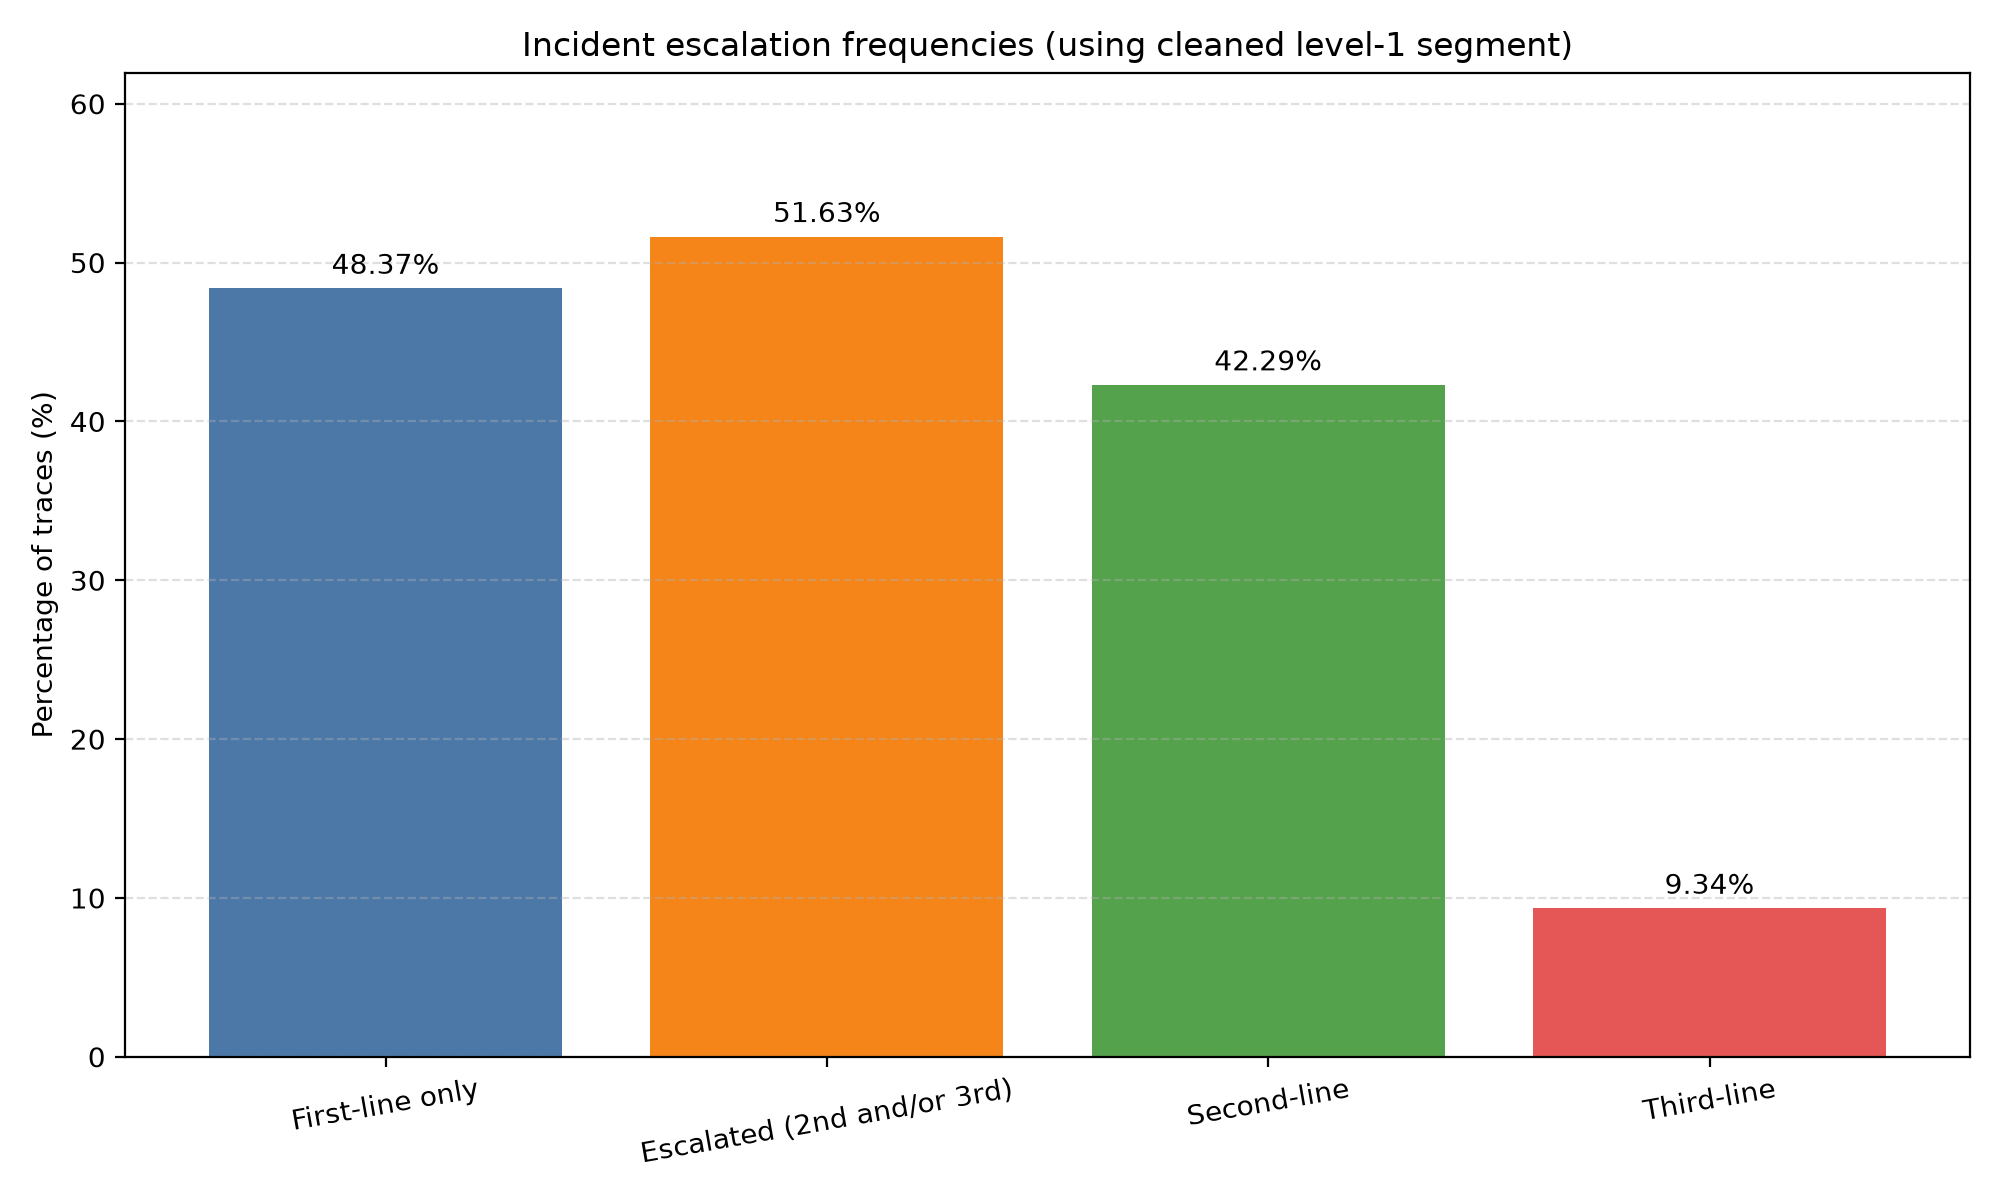
\includegraphics[width=0.9\textwidth]{pictures/escalation_frequency_cleaned.png}

This recalculation reveals a paradigm shift in understanding the IT incident management process at Volvo IT Belgium: the unfiltered events log suggested that the first line successfully resolved the majority of issues (approximately 60.18\%); however, once the artificial inflation caused by instantaneous system tickets is stripped away, the operational reality emerges: more than half of all incidents (51.63\%) require escalation to higher support tiers. This finding motivates further analysis to better understand potential inefficiencies.

Also, after this initial filtering of non-human-handled incidents, we can observe a pretty different distribution of traces duration times for the first-level segment.


    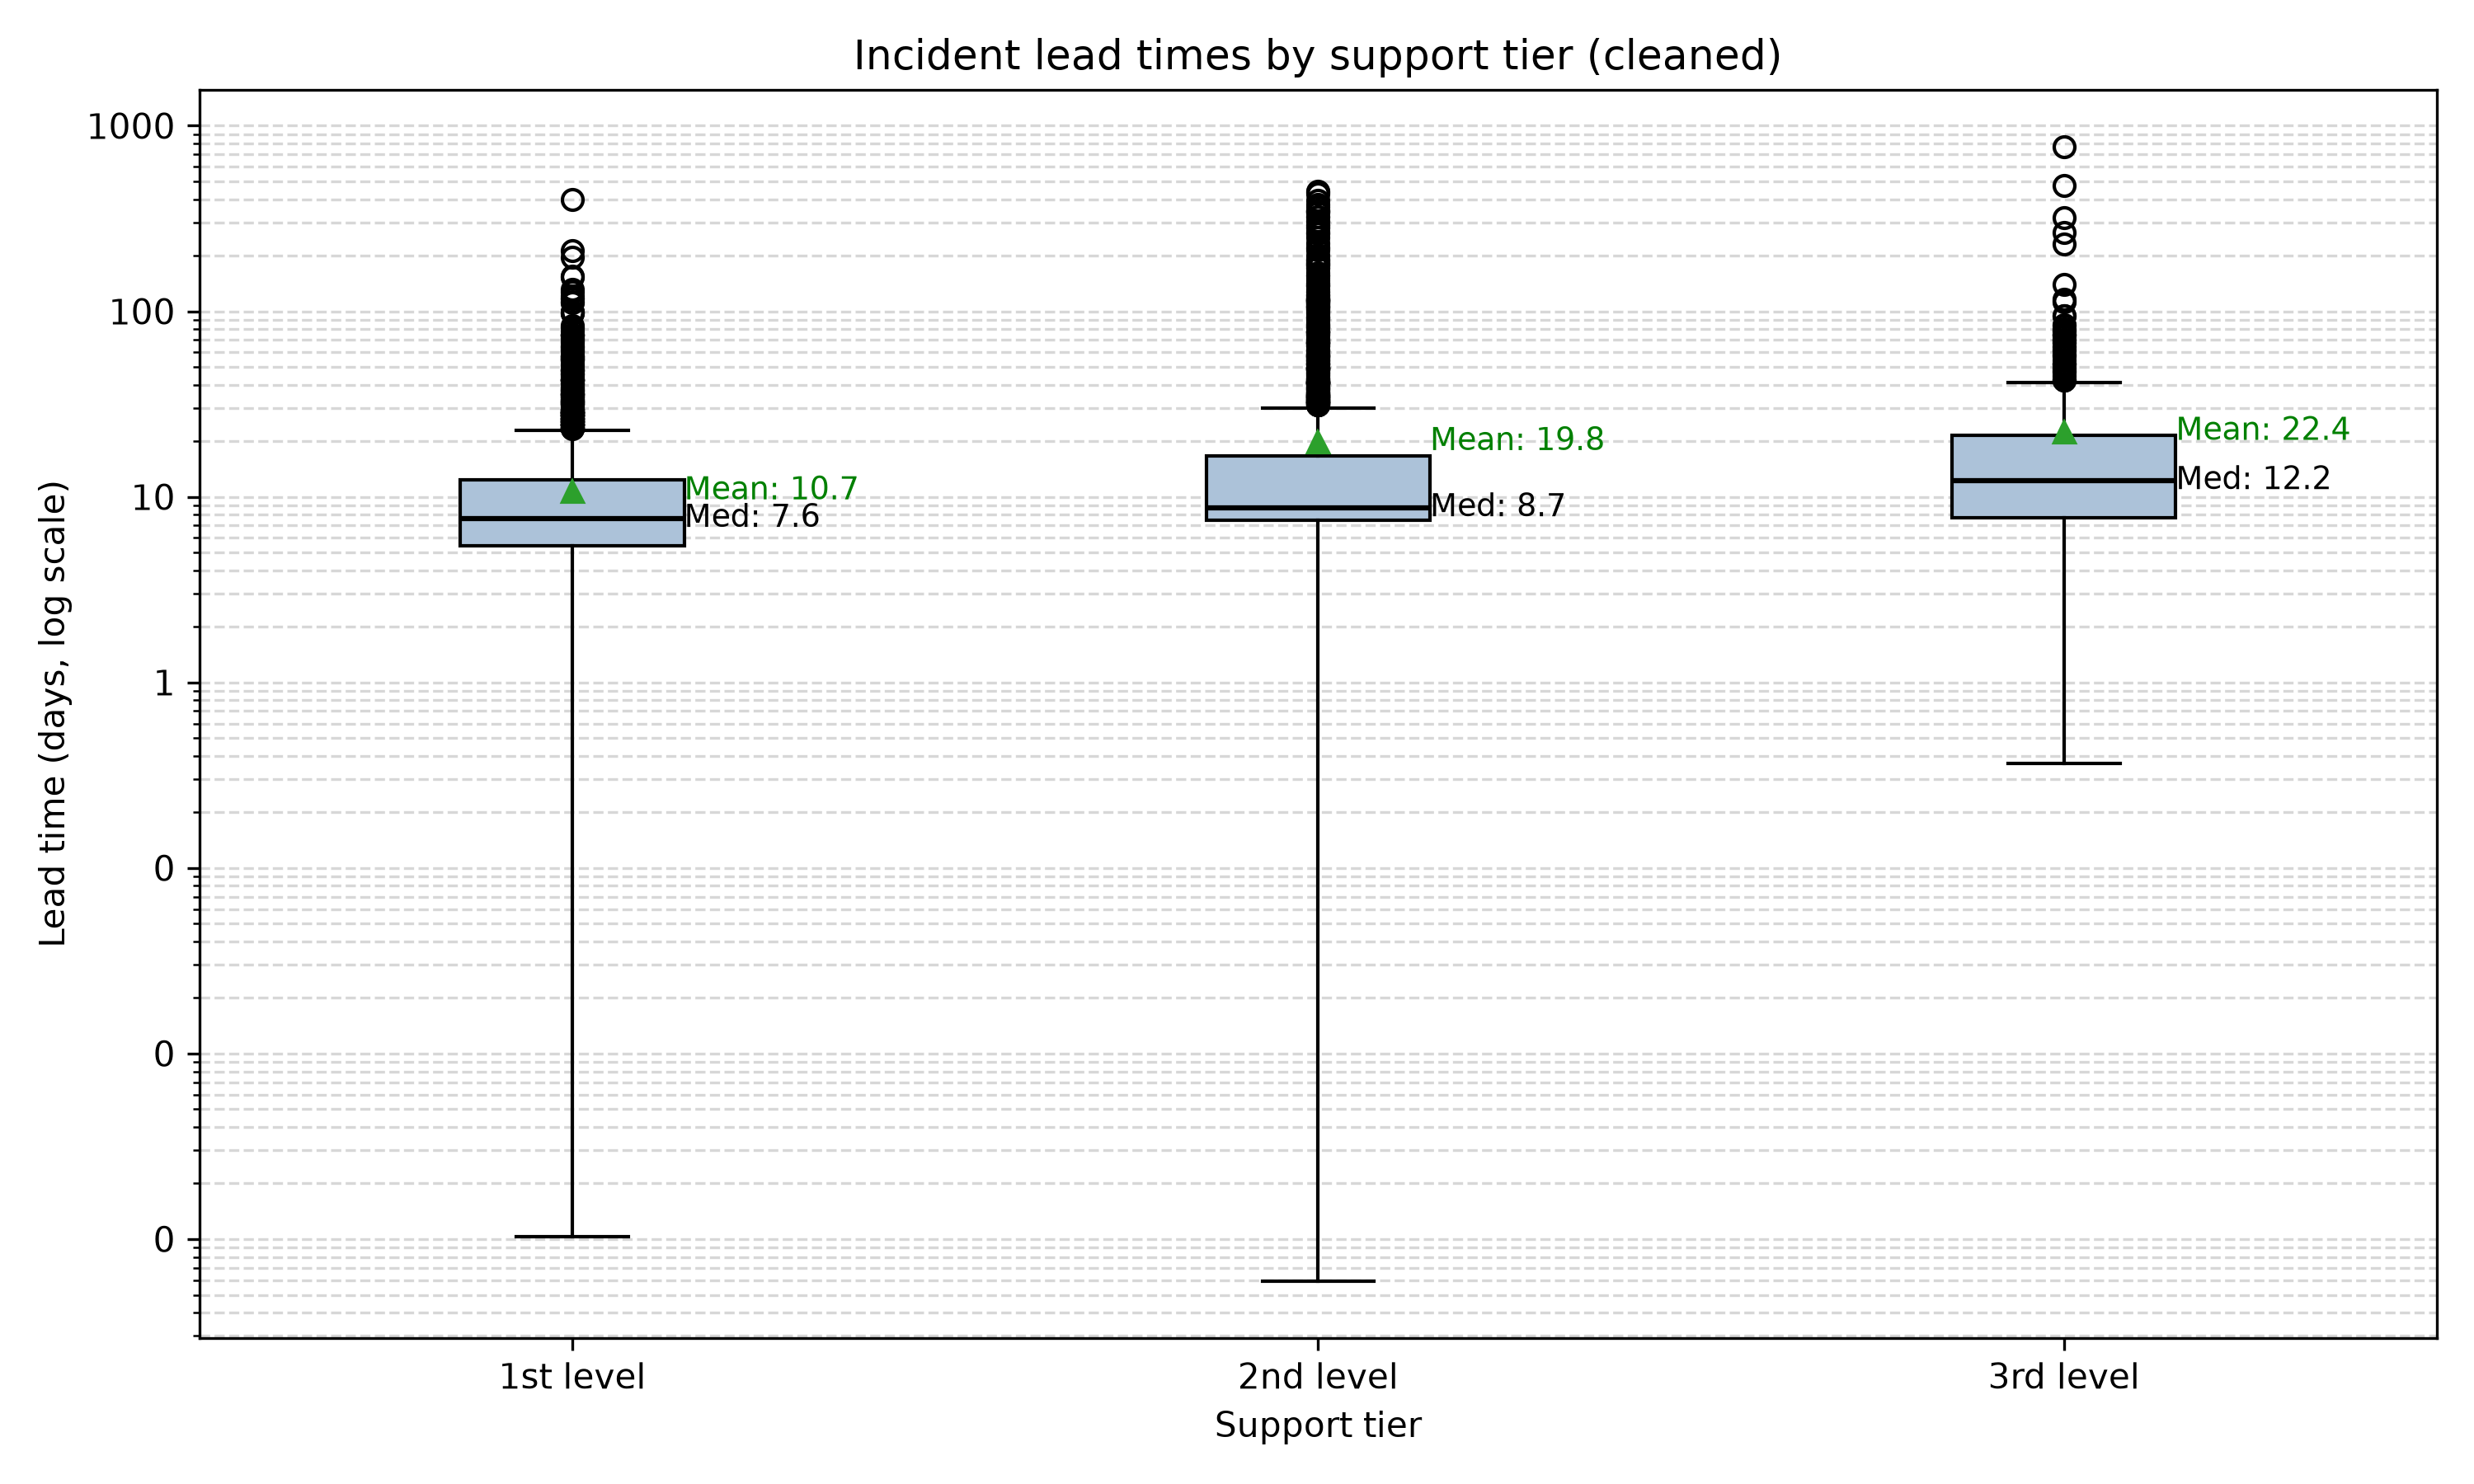
\includegraphics[width=0.9\textwidth]{pictures/lead_time_distribution_cleaned.png}

All the scripts used for the dataset filtering and for the data visualization are available in \texttt{cleaning.py} and \texttt{time\_duration\_stats\_segments.py}.

\subsection{Ping-pong behaviour analysis}

In the present scenario, a ``ping-pong'' behaviour occurs when a ticket is repeatedly reassigned back and forth between two support groups without progressing toward resolution. To isolate and quantify these inefficient dynamics, an algorithm that scans the ordered sequence of events within each trace has been created; it aims at processing events in contiguous blocks of three $(e_i, e_{i+1}, e_{i+2})$. A ping-pong pattern is formally registered if and only if the following logical condition is met:
\begin{center}
    \texttt{org:group($e_i$) == org:group($e_{i+2}$) \textbf{AND} org:group($e_i$) $\neq$ org:group($e_{i+1}$)}
\end{center}

When this $A \rightarrow B \rightarrow A$ cycle is detected, the algorithm records the specific pair of teams involved and calculates the total duration of the ping-pong. This duration is computed as the difference in timestamps between the return transfer ($e_{i+2}$) and the initial assignment to the originating team ($e_{i}$), effectively capturing the full amount of time lost in the redundant process. To focus on the most critical bottlenecks, the extracted metrics have been filtered using a 90th percentile threshold, isolating only the worst pairs across the three segments (using the cleaned version of the first-level log).

    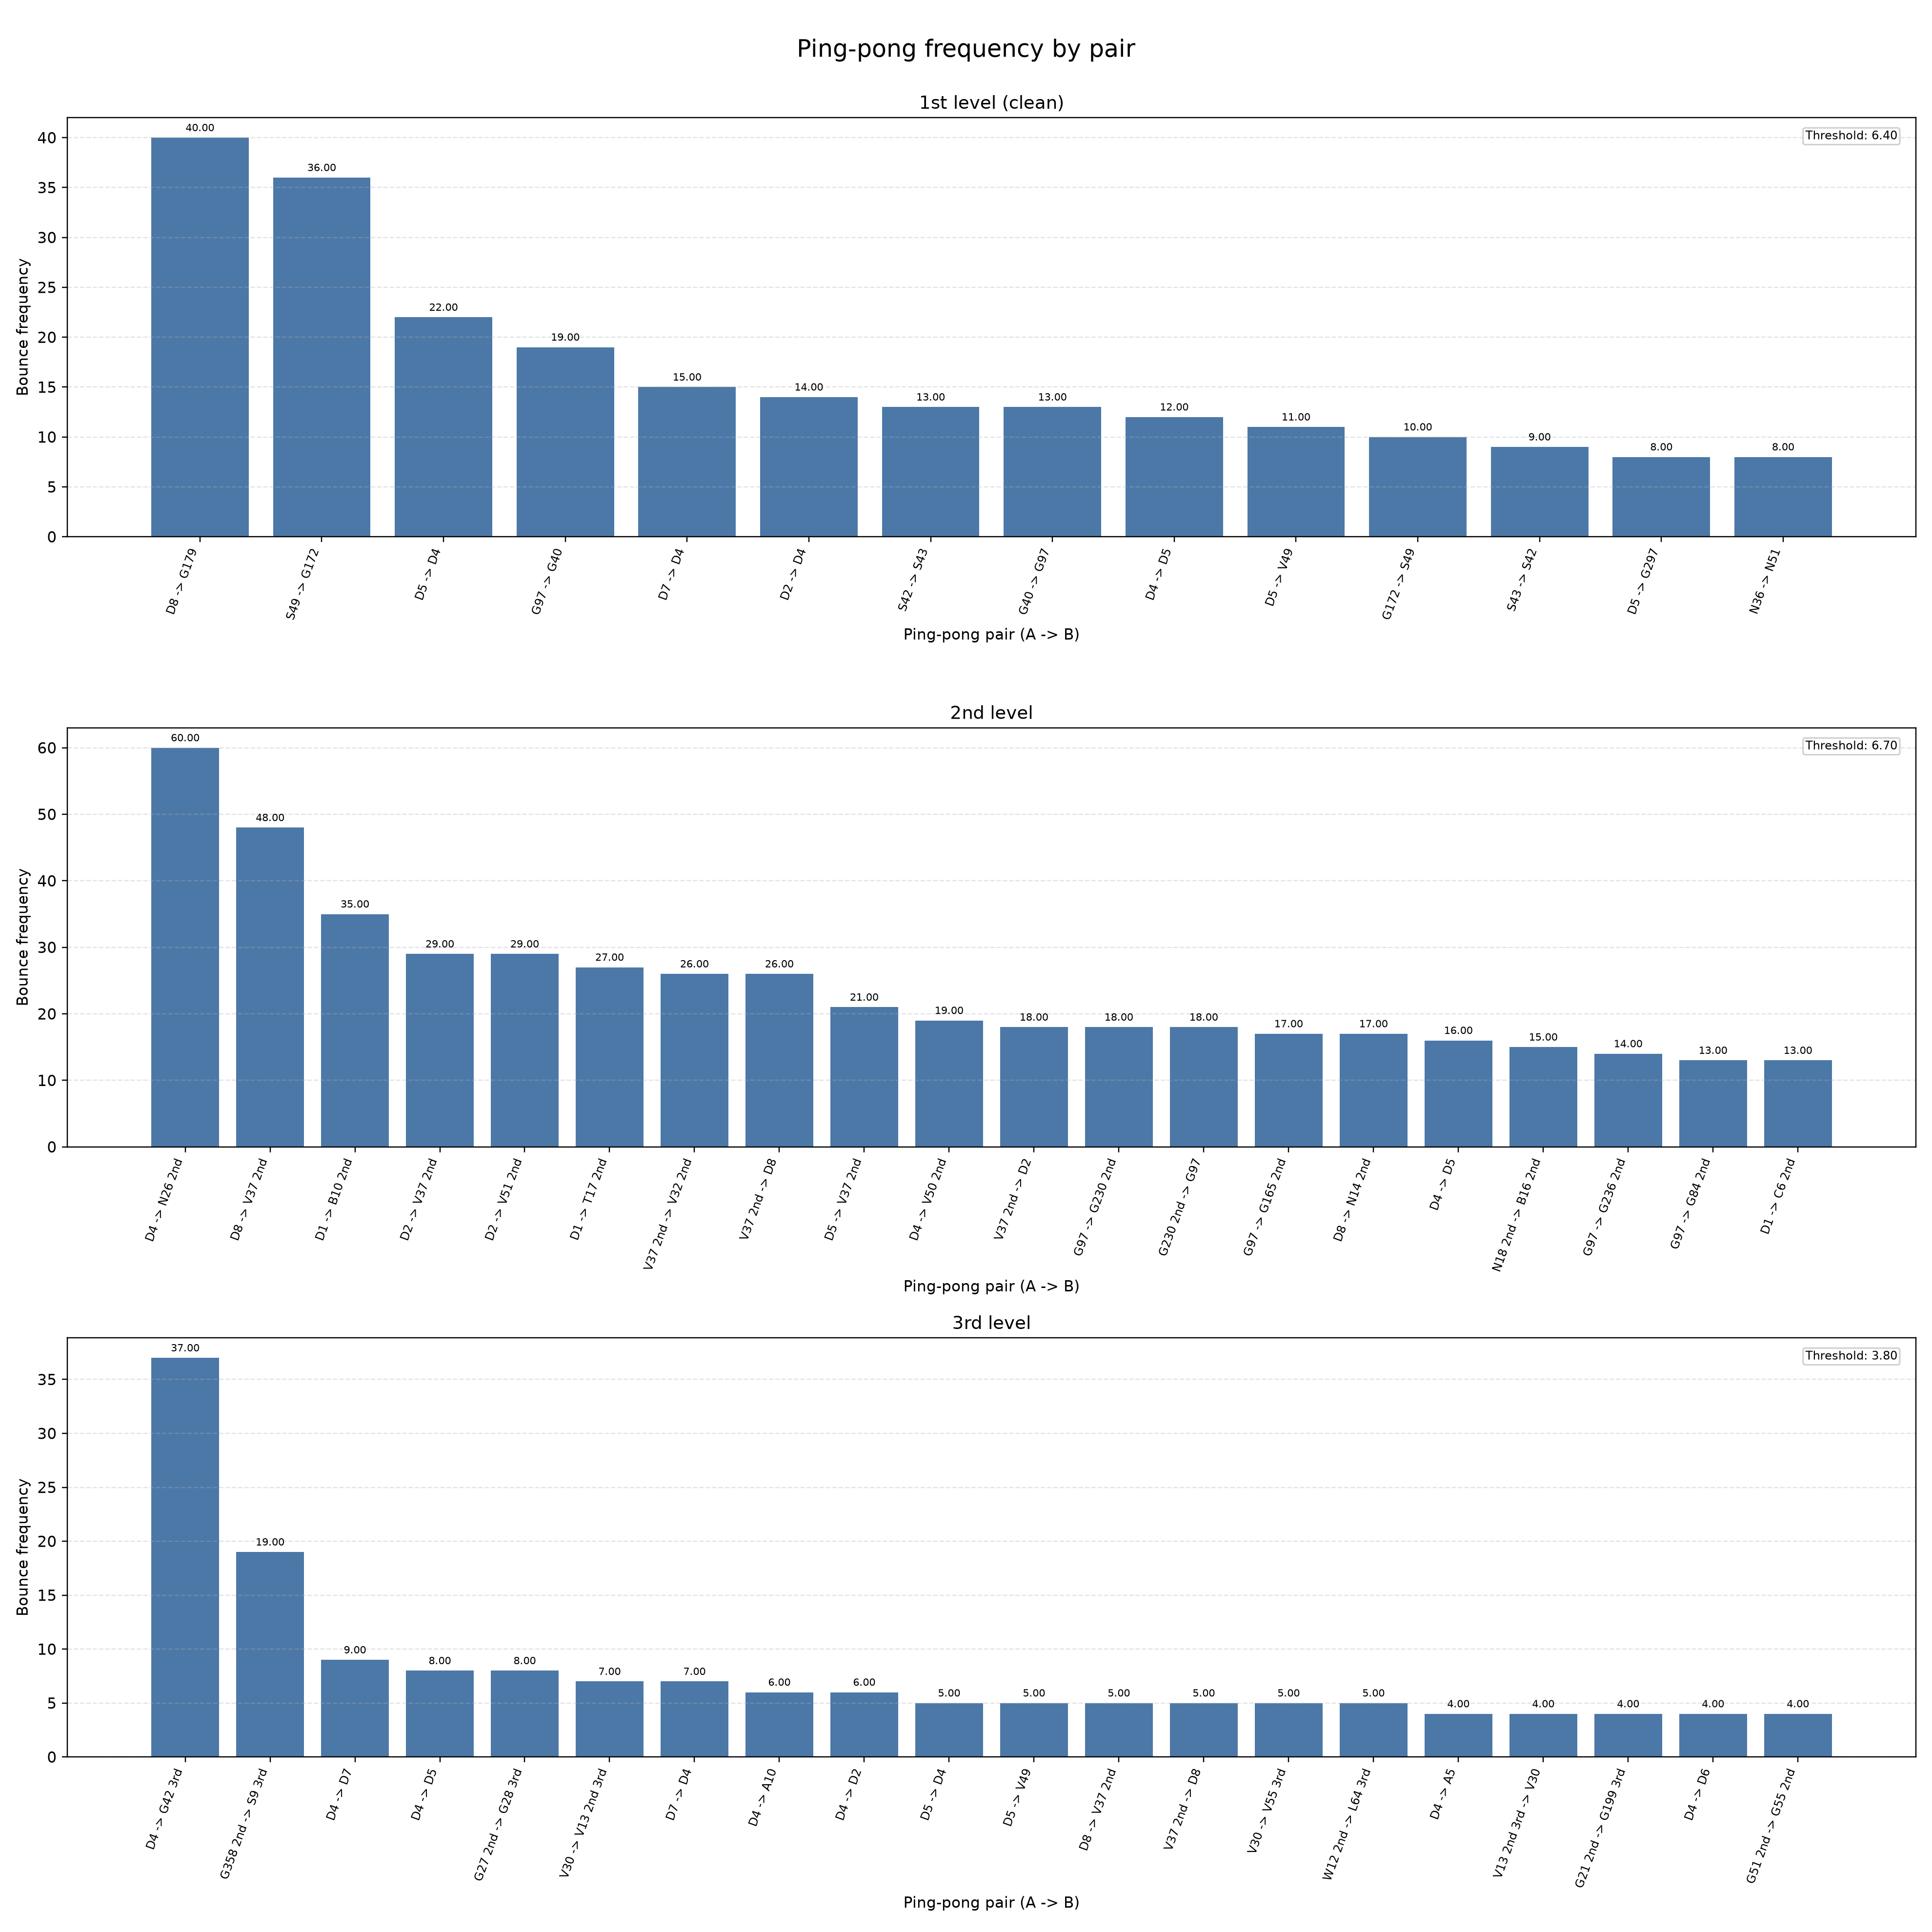
\includegraphics[width=0.9\textwidth]{pictures/pingpong_frequency_distribution_all_segments.png}
    
The frequency distribution reveals a high volume of redundant handovers across all tiers, but the second-level segment exhibits the most critical situation. The pair \texttt{D4 $\rightarrow$ N26 2nd} is the worst of the second level with 60 distinct bounces. While frequency indicates the volume of possible misrouted work, it does not necessarily reflect the severity of the delay. To evaluate the actual impact of ping-pongs, the cumulative lost time for each team pair was aggregated.

    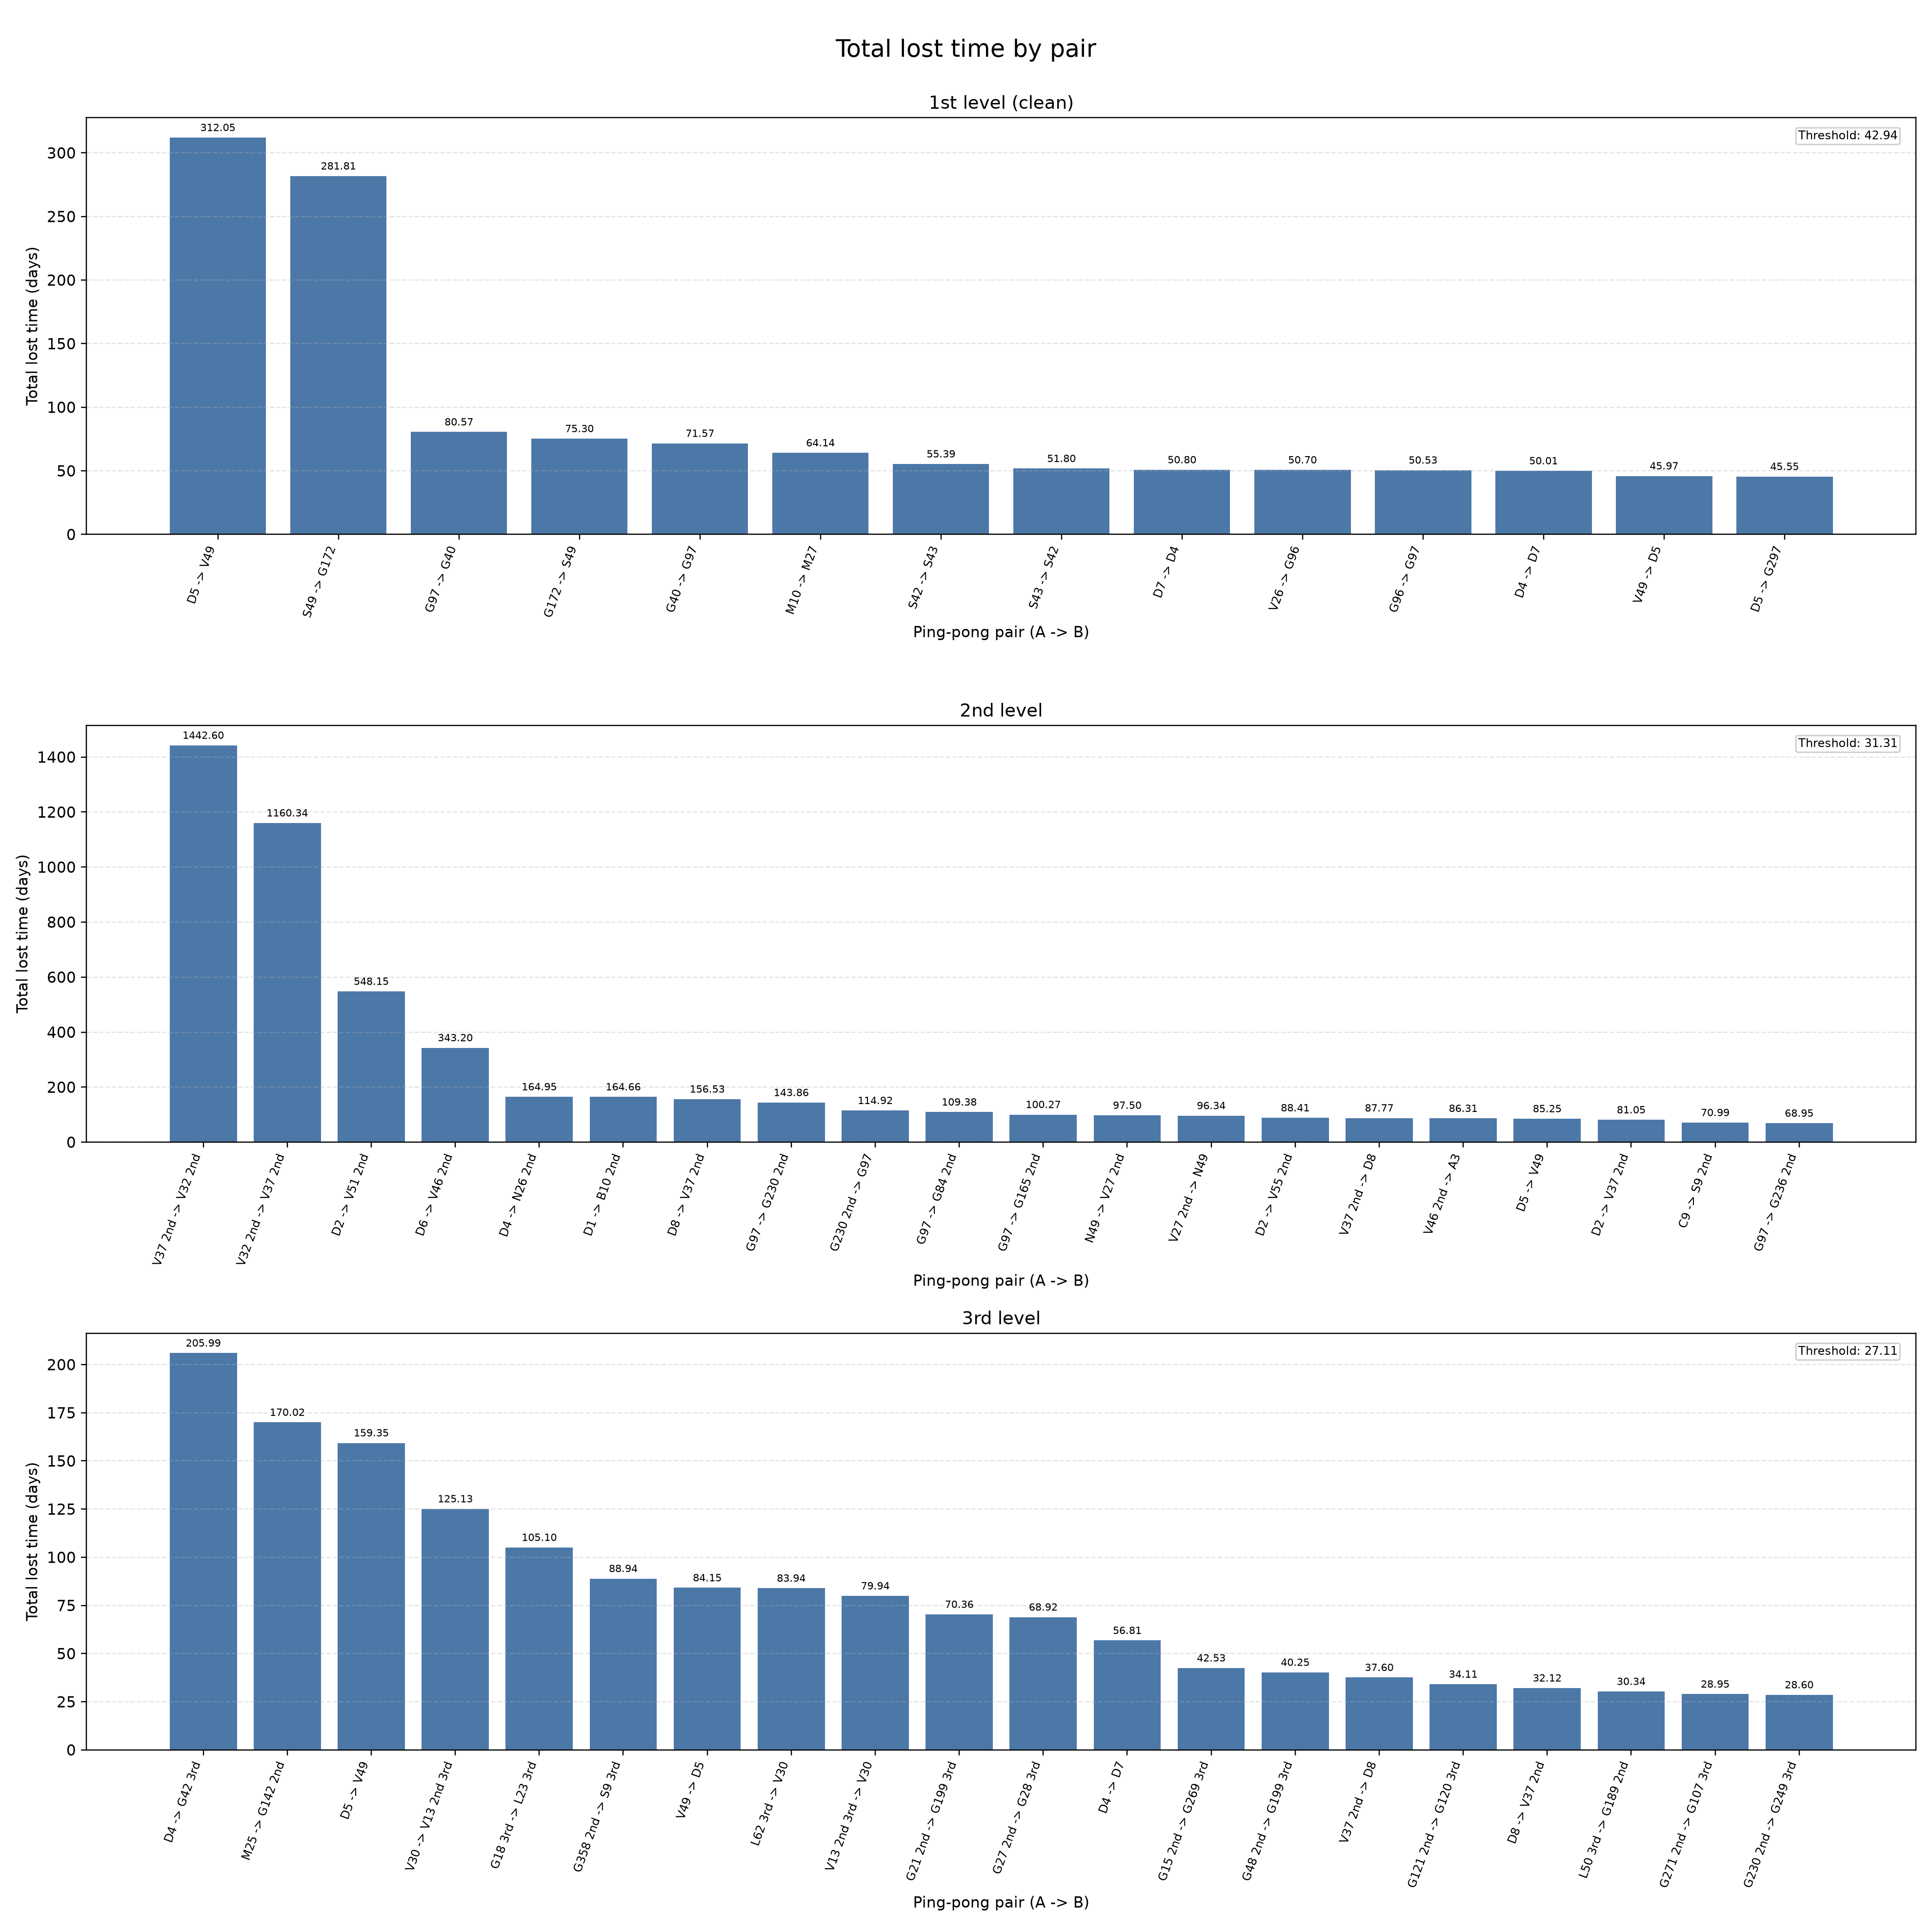
\includegraphics[width=0.9\textwidth]{pictures/pingpong_total_lost_time_distribution_all_segments.png}

The temporal analysis exposes a critical operational failure within the second-line support. The interaction between \texttt{V37 2nd} and \texttt{V32 2nd} generated an overwhelming 1442 days of accumulated wait time. This result implies that tickets routed to \texttt{V32 2nd} may remain without any progress for extended periods before being inevitably rejected and sent back to \texttt{V37 2nd} and this is something that happens for a huge number of pairs. This confirms that while the first line handles higher volumes of tickets, the most damaging operational delays occur deep within the specialized escalation tiers. To better investigate these findings and formulate targeted recommendations, it is necessary to identify the specific groups responsible for initiating these unproductive cycles.

    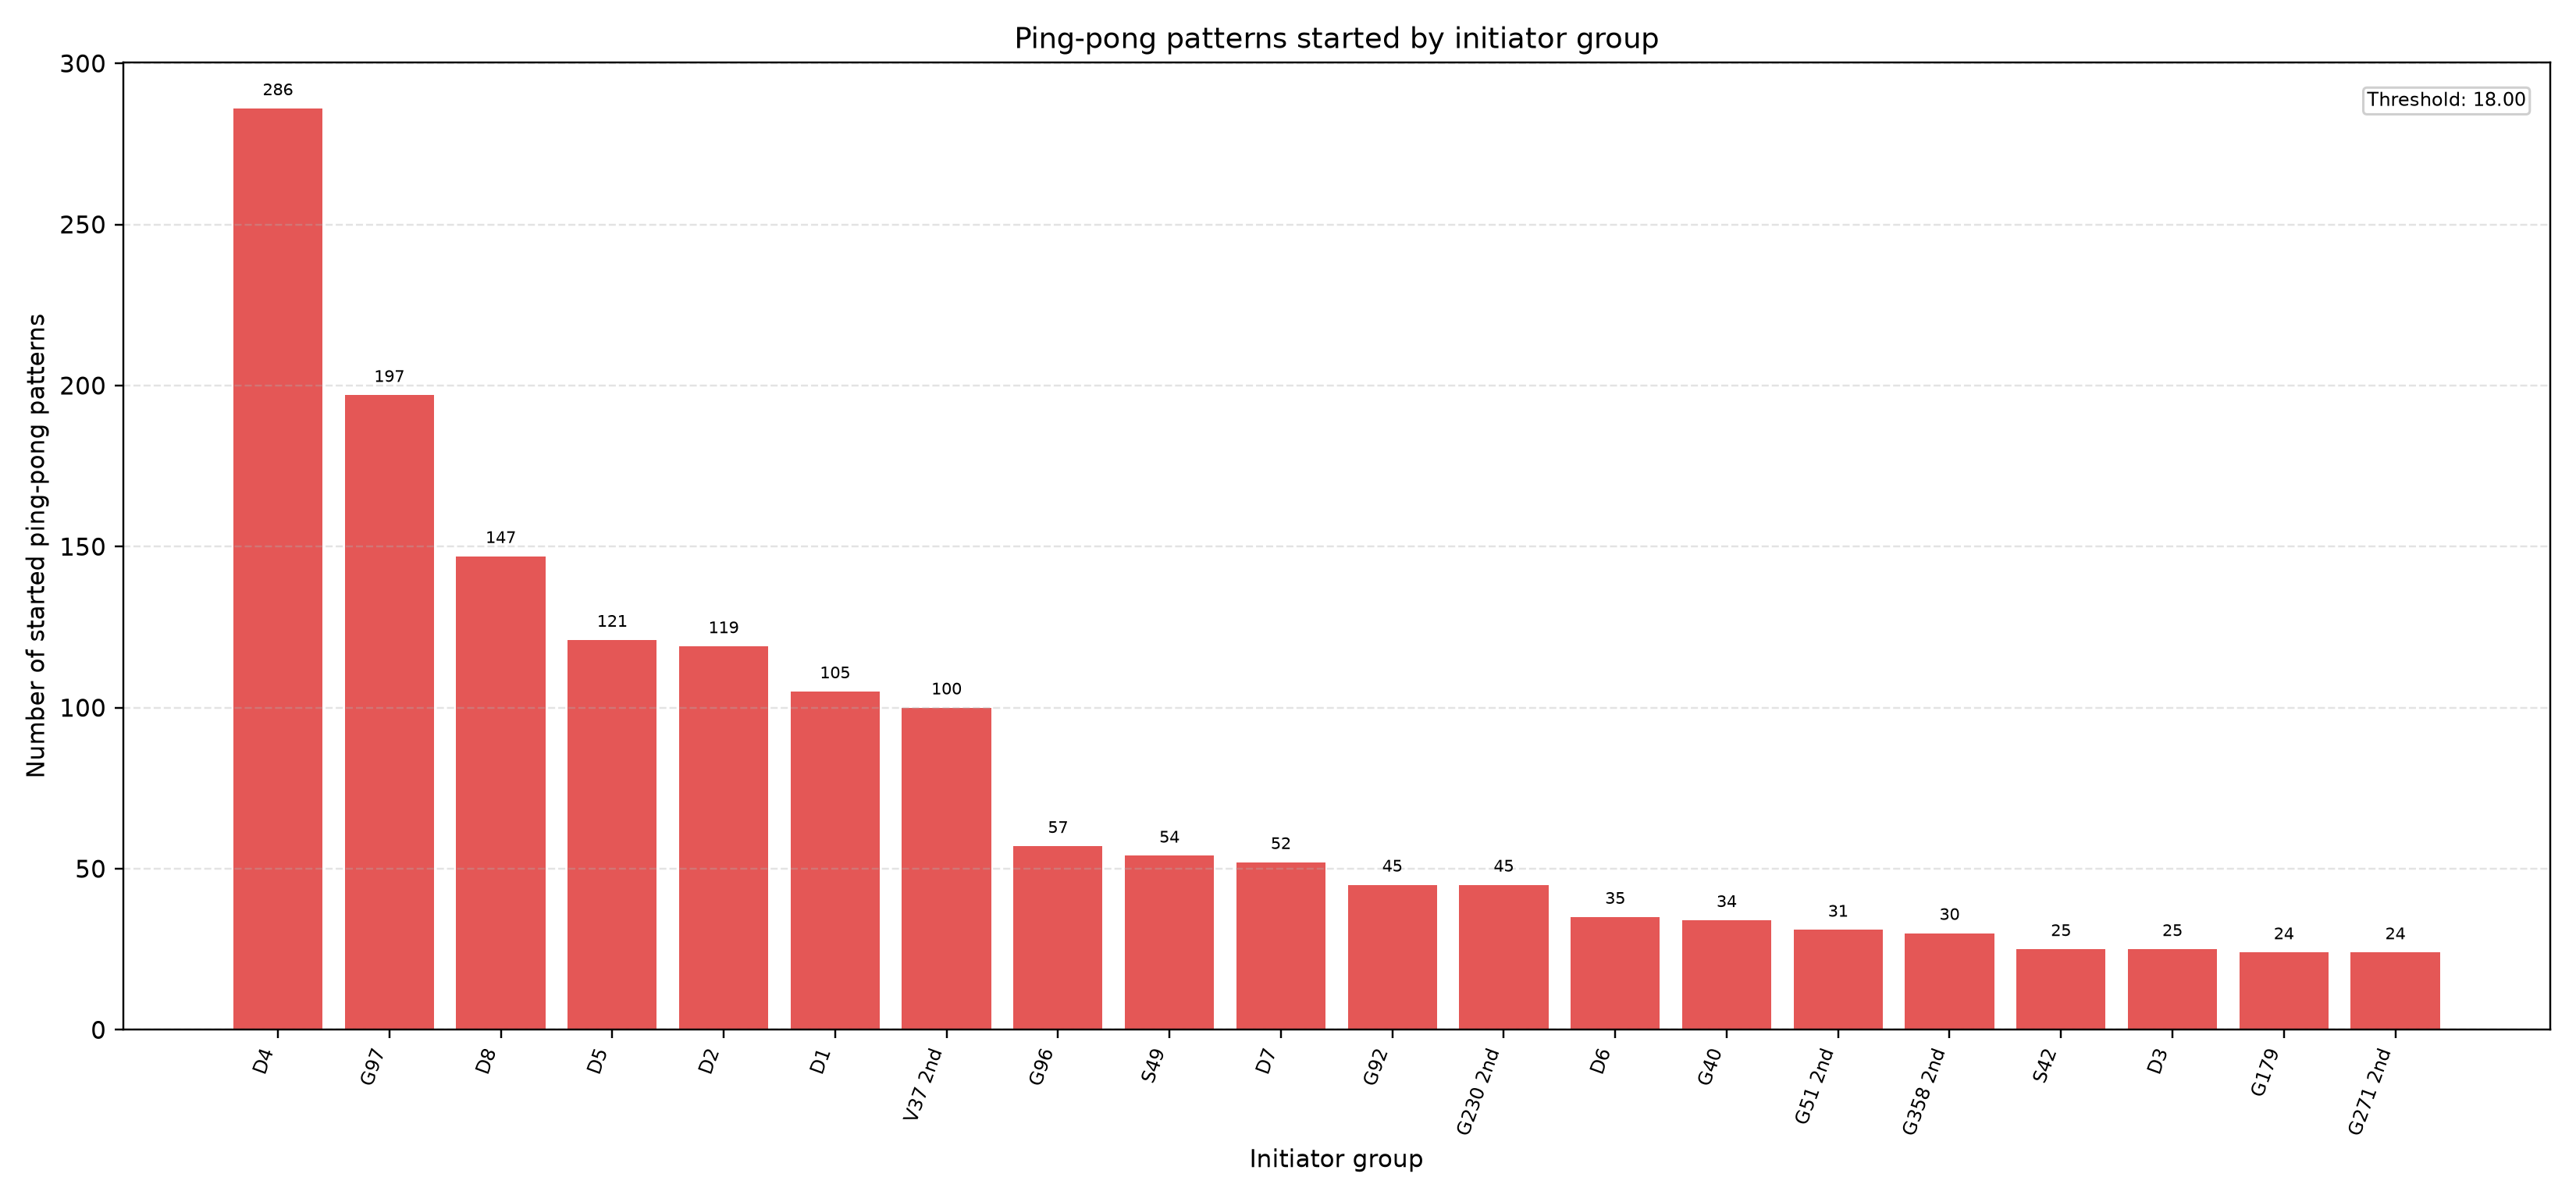
\includegraphics[width=0.9\textwidth]{pictures/pingpong_initiator_distribution_all_segments.png}
    
The above graphic aggregates the total number of ping-pong patterns triggered by each one the worst groups (the sender who eventually receives the ticket back). The distribution identifies group \texttt{D4} as the absolute worst offender, having initiated 286 redundant cycles, followed by G97 and D8. These results strongly suggest that operators belonging to these groups either lack the necessary diagnostic tools to route tickets correctly on the first attempt or operate under wrong procedure guidelines, systematically causing all this incident bouncing behaviour.

Finally, the average duration of all incidents has been calculated focusing on the previous segmentation and trying to highlight a significant difference between the traces containing at least one ping-pong and the "clean" ones.

\begin{table}[h]
\centering
\begin{tabular}{lrrrr}
\hline
Segment & Mean w/ PP (d) & Mean w/o PP (d) & Traces w/ PP & Traces w/o PP \\
\hline
1st level (clean) & 17.68 & 9.95 & 283 & 2535 \\
2nd level & 31.70 & 14.97 & 708 & 1756 \\
3rd level & 32.95 & 17.00 & 186 & 358 \\
\hline
\end{tabular}
\end{table}

\begin{table}[h]
\centering
\begin{tabular}{lrrrr}
\hline
Segment & Med w/ PP (d) & Med w/o PP (d) & Traces w/ PP & Traces w/o PP \\
\hline
1st level (clean) & 11.03 & 7.61 & 283 & 2535 \\
2nd level & 13.29 & 8.38 & 708 & 1756 \\
3rd level & 13.51 & 10.91 & 186 & 358 \\
\hline
\end{tabular}
\end{table}

These findings agree with the initial hypothesis raised by Volvo IT Belgium regarding the impact of ping-pong behaviour on operational performance: the evidence confirms that redundant handovers are primary causes of delays and structural inefficiency within the incident management lifecycle. The script used in this section is available in \texttt{pingpong\_handover\_segments.py}

\subsection{Cross-department conformance analysis}

To evaluate whether the ping-pong inefficiencies detected in the previous section correlate with any procedural deviation, a cross-department conformance analysis has been conducted. Since Volvo IT Belgium didn't provide a formal \textit{To-Be} model for incidents management, an ``ideal'' reference model has been empirically discovered from the data. 

This analysis uses a unified dataset combining the cleaned 1st-level log (free of automated noise) with the 2nd and 3rd-level logs, resulting in 5826 incident traces. The reference model has been generated using the \textbf{Heuristics Miner} algorithm to catch all the possible transitions of \texttt{concept:name} values but exclusively on the subset of traces that do not contain any ping-pong patterns. This makes it possible to measure conformance against the pure procedural lifecycle. A Petri net representing the extracted model is included below.

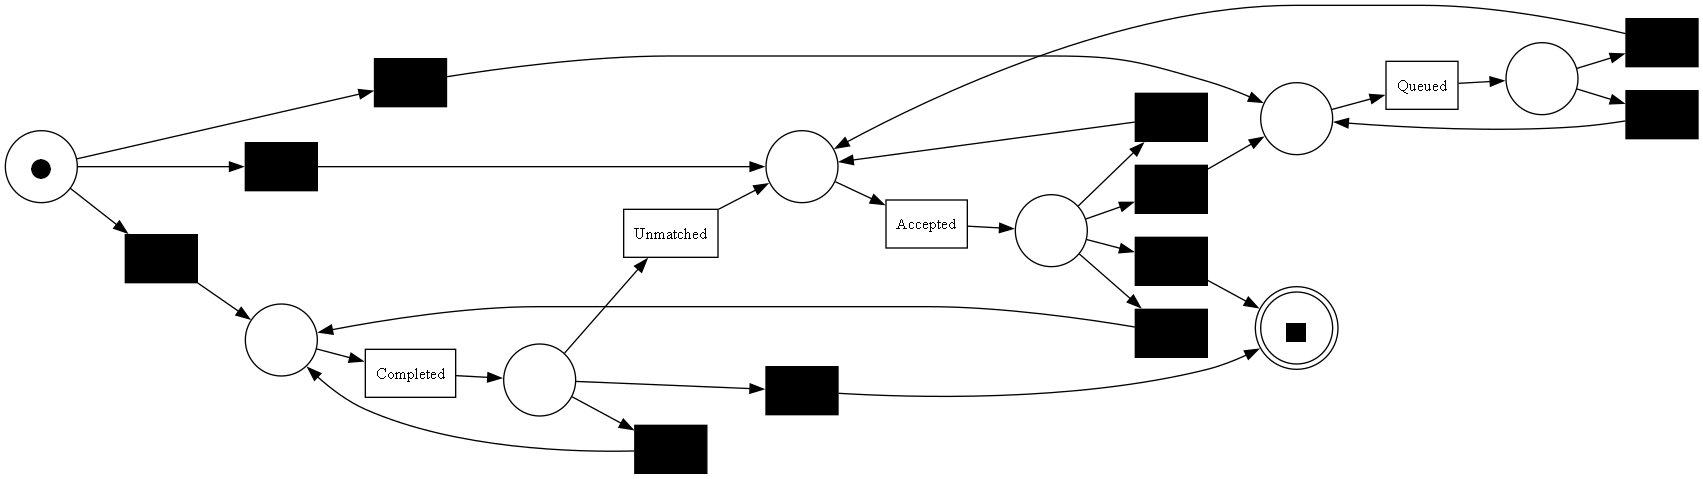
\includegraphics[width=1\textwidth]{pictures/reference_model_combined_no_pingpong.png}


In order to match the requests of this project, it seemed interesting to measure the impact of the two worst-performing groups (\texttt{D4} and \texttt{G97}). For this reason, the unified dataset $D$ (cleaned 1st-level segment $\cup$ 2nd-level segment $\cup$ 3rd-level segment) has been partitioned into mutually exclusive variants using $T_{D4}$ and $T_{G97}$, which are the sets of traces involving these respective groups. Since these groups belong to different organization lines, no trace with both of them is present in the dataset. So $D$ was divided into three strict variants: 
\begin{itemize}
    \item $T_{D4} \setminus T_{G97}$ (traces involving D4 but not G97);
    \item $T_{G97} \setminus T_{D4}$ (traces involving G97 but not D4);
    \item $(T_{D4} \cup T_{G97})^c$ (the baseline involving neither).
\end{itemize}

The conformance of these variants against the ideal model was evaluated using Token-Based Replay (see \texttt{fitness\_variants.py}).

\begin{table}[H]
    \centering
    \begin{tabular}{@{}lccc@{}}
        \toprule
        \textbf{Variant subsets} & \textbf{Traces} & \textbf{Percentage of fitting traces} \\ \midrule
        Involving \texttt{D4} (not \texttt{G97}) & 210 & 93.33\% \\
        Involving \texttt{G97} (not \texttt{D4}) & 950 & 82.53\% \\
        Others (neither \texttt{D4} nor \texttt{G97}) & 4666 & 92.20\% \\ \bottomrule
    \end{tabular}
\end{table}

The results highlight that, despite being the primary initiator of ping-pong delays, group \textbf{D4} achieved a percentage of fitting traces (93.33\%) that actually surpasses the baseline (92.20\%). This indicates that D4 is responsible for continuous bouncing of tickets that is procedurally valid within the system's state machine and seems to have no effect on conformance. They follow the ticketing rules, yet often passing them to other departments.

In contrast, group \textbf{G97} has a lower conformance level. With 82.53\% of their traces fitting the model, they lag behind the company average. Unlike D4, G97's inefficiency is not merely organizational; it is procedural. They sometimes violate the standard lifecycle of the tickets, executing rare state transitions and moving further away from the ideal model.

\newpage

\section{Conclusions}

The application of process mining techniques to the Volvo IT dataset provided sufficient answers to the core operational challenges of the incident management process. 

First, the analysis demonstrated that incidents escalated to second and third-line support intrinsically take longer resolution times. While escalations are sometimes necessary, the structural delay they introduce confirms that maximizing first-line resolution must remain a primary business objective to prevent system bottlenecks.

Second, the detection of ping-pong patterns has made it possible to isolate the specific support groups responsible for initiating redundant handovers. The temporal data definitively links these cyclic routing behaviours to significantly longer incident management times and accumulated delays. 

However, cross-department conformance checking revealed a paradox: generating a high volume of ping-pongs does not necessarily imply violations of the prescribed process lifecycle. Groups can be highly inefficient while remaining compliant with the system's state transitions.

Finally, the current event log lacks granular metadata detailing the actual IT problem typology (e.g., hardware failure, network outage, software bug). To enable a better performance assessment and deeper root-cause analysis, it could be recommended to enhance the VINST logging system to capture incident categories at the time of creation. Incorporating this problem-type metadata would allow future investigations to benchmark support groups based on task complexity, making it possible to develop better routing rules and to plan targeted operator training.

\subsubsection*{An unresolved anomaly}
A curiosity emerged during the temporal analysis of ping-pongs (scripts in \texttt{pingpong\_yearly.py}), highlighting an anomaly that remains difficult to fully explain without additional contextual data.


    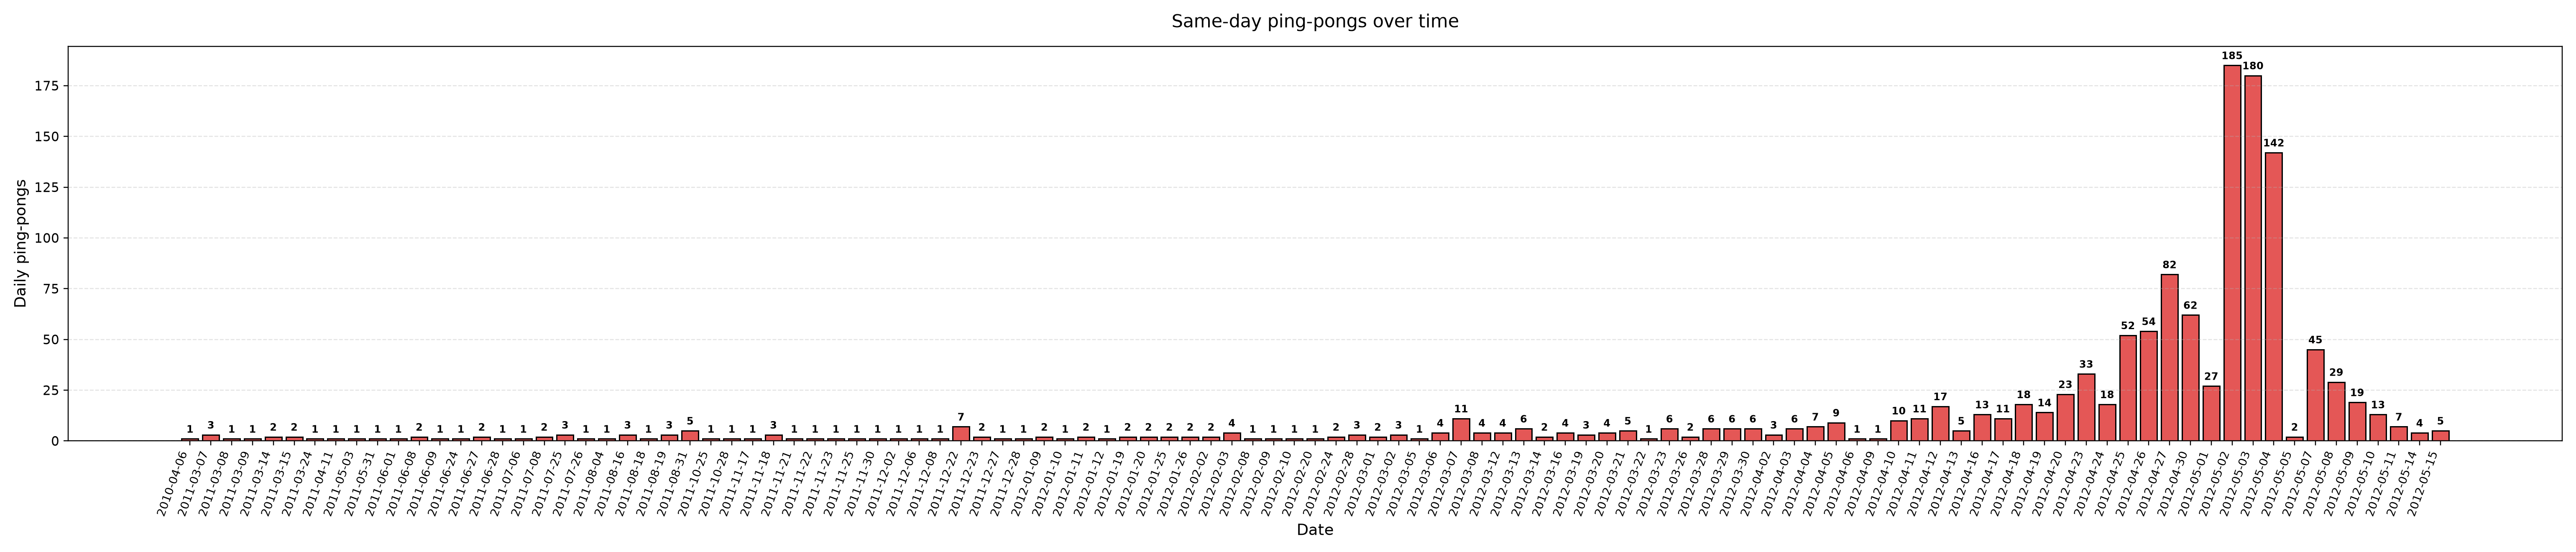
\includegraphics[width=1\textwidth]{pictures/pingpong_yearly_distribution.png}

     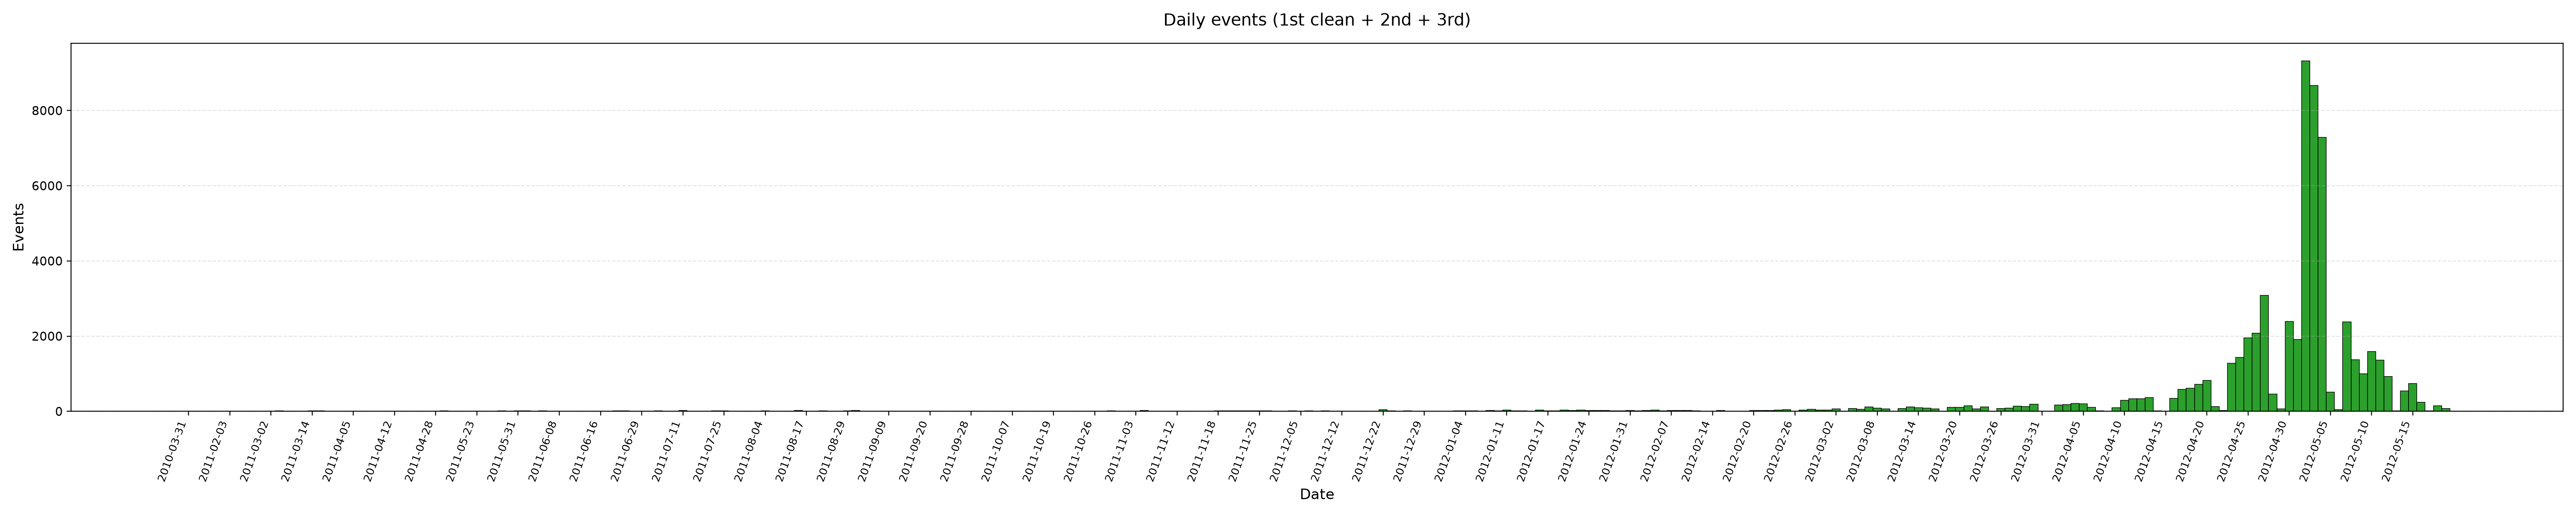
\includegraphics[width=1\textwidth]{pictures/event_yearly_distribution_segments.png}

For the vast majority of the observed period, same-day ping-pongs (instances where a ticket is bounced $A \rightarrow B \rightarrow A$ within 24 hours) represented mere operational background noise. However, between April and May 2012, the system experienced a peak at over 180 same-day ping-pongs within a single 24-hour window. 

Such a spike suggests that something like a massive bulk-routing error, a major infrastructure outage generating a flood of identical tickets or a temporary automated routing bug in the VINST system might had happened. Unfortunately, without further qualitative data, it is impossible to identify the cause of this isolated crisis. This remains a curiosity for future research, highlighting the necessity of integrating process mining findings with operational and business context.

\section{Code reference}

The complete source code, including data preparation scripts, the algorithmic implementation for ping-pong detection, and the conformance checking evaluations using PM4Py, is available for review at the following GitHub repository:

\url{https://github.com/gianlucapironato/BIS-2026-Unimi}

\end{document}